\documentclass[
enabledeprecatedfontcommands, % \sc erlauben
12pt,                  % Schriftgroesse [10,11 oder 12pt]
a4paper,               % Papierformat
titlepage,             % Es soll eine Titelseite verwendet werden!
headsepline,
%draft,                % schnelle Vorschau
%abstracton,           % Abstract oder nicht?
appendixprefix,        % Mit dieser Option wird das A, B etc. vor den Kapiteln im Anhang aktiviert.
headings=normal,       % Gibt die Groesse der Ueberschriften an. Zulr Wahl stehen smallheadings, normalheadings und bigheadings.
parskip=half*,         % Mit dieser Option beeinflusst man die Absatzformatierung.
captions=tableheading, % Setzt die Tabellenbeschriftung ueber die Tabelle.
chapterprefix,         % Mit dier Option schaltet man ein, dass vor jedes Kapitel 'Kapitel 1' etc. geschrieben wird.
twoside,               % Mit dieser Option gibt man an, ob man ein zweiseitiges Format (--> Buch) wuenscht oder nicht.
BCOR=15mm,			   % Bindungskorrektur
%liststotoc            % Bewirkt, dass dem Inhaltsverezeichnis das Abbildungs- und Tabellenverzeichnis hinzugefuegt wird.
bibliography=totoc,
numbers=noenddot,
version
]{scrbook}

\usepackage{ucs}
%\usepackage[latin1]{inputenc}
\usepackage[UTF8]{inputenc}
\usepackage[T1]{fontenc}
\usepackage[pdftex]{graphicx}
\graphicspath{{./images/}}
\usepackage{color}
\usepackage[ngerman]{babel}
\usepackage{subfigure}
\usepackage[automark]{scrpage2}  % Kopf- und Fusszeilen

\usepackage{booktabs}
\usepackage{hyperref}
\usepackage{siunits}  % fuer ein schoenes mu
\usepackage{upgreek}

%% MATHEMATISCHE NOTATION:
%\usepackage{dsfont}
%\usepackage{amssymb}
\usepackage{amsmath}
\usepackage{amstext}
\usepackage{units}

%% EINBINDEN VON QUELLCODE / DEF VON ALGORITHMEN:
\usepackage{verbatim}
%\usepackage[vlined]{algorithm2e}
\usepackage{algorithm}
\usepackage{algorithmic}
\floatname{algorithm}{\footnotesize Algorithmus}
\usepackage{booktabs}

%% LITERATURANGABE:
\usepackage{bibgerm}

%% TIKZ
\usepackage{tikz,pgfplots}
\usepackage{textcomp}
\usepackage[european]{circuitikz}

%% table footnotes
\usepackage{footnote}
\makesavenoteenv{tabular}
\makesavenoteenv{table}

\usepackage{listings}

%% ORIGINAL PACKAGE DEFINES:
% \renewcommand{\capfont}{\normalfont}
% \renewcommand{\caplabelfont}{\normalfont}
% \renewcommand{\descfont}{\sffamily\bfseries}
% \renewcommand{\headfont}{\slshape}
% \renewcommand{\pnumfont}{\normalfont}
% \renewcommand{\sectfont}{\sffamily\bfseries}

\renewcommand{\descfont}{\bfseries}
\renewcommand{\sectfont}{\bfseries}

\setkomafont{captionlabel}{\bfseries\footnotesize}
\setkomafont{caption}{\footnotesize}
\renewcommand{\headfont}{\bfseries}
\renewcommand{\figurename}{Abb.}
\renewcommand{\tablename}{Tabelle}

\renewcommand*{\titlepagestyle}{empty}

\newcommand{\lorem}{Lorem ipsum dolor sit amet, consectetur adipiscing elit, sed do eiusmod tempor incididunt ut labore et dolore magna aliqua. Ut enim ad minim veniam, quis nostrud exercitation ullamco laboris nisi ut aliquip ex ea commodo consequat. Duis aute irure dolor in reprehenderit in voluptate velit esse cillum dolore eu fugiat nulla pariatur. Excepteur sint occaecat cupidatat non proident, sunt in culpa qui officia deserunt mollit anim id est laborum.}

%% ------------------------------------------------------------------------
%%  EIGENE DEFINITIONEN
%% ------------------------------------------------------------------------

%% RANDABSTAENDE:
\usepackage{calc}
\usepackage{geometry}
\usepackage{pdfpages}	%kann Titelseite als pdf einbinden
\geometry{left=3.0cm, right=2.5cm}%, top=1.0cm}%bottom=1.0cm}%, top=4.0cm}
\addtolength{\textheight}{2.7cm}
\setlength{\skip\footins}{10mm}

\usepackage[%
       final,%
       activate,%
       verbose=true]{microtype}
\usepackage{%
       fixltx2e,%
       mparhack%
}

% schönere Abbildungen
\usepackage{mwe}
\newcommand*{\quelle}[1]{\par\centering\footnotesize Quelle:~#1}


%% FARBEN:
\definecolor{Ocean}{cmyk}{1,0,0.2,0.78}
\definecolor{Grey}{cmyk}{0,0,0,0.6}
\definecolor{ULGray}{cmyk}{0,0,0.03,0.1}

%% KOPF- UND FUSSZEILEN:
\pagestyle{scrheadings}
%\chead{}
%\ihead{\headmark}
%\ohead[\pagemark]{\pagemark}
%\cfoot[]{}
\clearscrheadfoot
\rehead{\headmark}
\lehead{\pagemark}
\lohead{\headmark}
\rohead{\pagemark}


\begin{document}
%\setlength{\headheight}{0pt}
%\pgfplotsset{width=10cm,compat=1.6}	%fuer Grafikbeschriftung der rechten Achse
\pgfplotsset{width=10cm,compat=1.6}	%fuer Grafikbeschriftung der rechten Achse

\tikzstyle{every pin}=[fill=white,draw=black,font=\footnotesize]	%Beschriftung der Marker

%% ------------------------------------------------------------------------
%% TITELSEITE
%% ------------------------------------------------------------------------

%\begin{titlepage}
%%\input{./otherincludes/Titelseite}
%%\input{./otherincludes/Titelseite_sf}
%\includepdf{./otherincludes/TitlePage-Monsterratte.pdf}
%\end{titlepage}


\thispagestyle{headings}
\pagenumbering{roman}
\begin{titlepage}
\includepdf{./otherincludes/TitlePage-BachelorMaster.pdf}
\end{titlepage}


%% ------------------------------------------------------------------------
%% VERZEICHNISSE ETC
%% ------------------------------------------------------------------------

%\thispagestyle{headings}
%\pagenumbering{roman}


\thispagestyle{empty}
\null\newpage
\thispagestyle{empty}
\thispagestyle{empty}

\vspace*{7cm}
Ich versichere an Eides statt, dass ich die vorliegende Arbeit selbstständig verfasst und\\
keine anderen als die angegebenen Quellen und Hilfsmittel benutzt habe.

\vspace*{3cm}
%\textcolor{red}{Unterschrift}\\
Lübeck, den \today



\thispagestyle{empty}
\null\newpage
\thispagestyle{empty}
\thispagestyle{empty}


\vspace*{6cm}
{\Huge \textbf{Danksagung} }
\vspace*{1cm}

Ich danke meinen Eltern für ihre tatkräftige Unterstützung während meines gesamten Studiums.

Speziellen Dank richte ich an Jan Haase, für die gute Betreuung dieser Arbeit, an Philipp Grothe, für die Hilfestellungen während der Arbeit und an Thore Kolms, welcher gleichzeitig mit mir an seiner Bachelorarbeit auf dem gleichen Themengebiet gearbeitet hat. Vielen Dank für die tolle Zusammenarbeit.

Danke auch an Stefan Tran und Adrian Beeck für das Korrekturlesen meiner Arbeit.



\chapter*{Kurzfassung}

Der Memristor ist ein stark diskutiertes Schaltungselement, welches die Eigenschaft besitzt einen variablen Widerstand anzunehmen. Bei Memristoren handelt sich um nichtflüchtigen Speicher. Seit der ersten Erwähnung des Memristors und neu angefacht durch die Entwicklung eines funktionierenden Prototypen, wird unter Experten darüber diskutiert, ob dieses neue fundamentale Schaltungselement die Zukunft der Speichermedien darstellt, oder nicht. Doch klar ist, dass auch noch heute, im Jahr 2020, noch lange nicht der Zenit der Memristoren erreicht ist und einige dieser Bausteine aus unterschiedlichen Gründen ihr mögliches Potential noch nicht ausgeschöpft haben. In der Praxis kommt es zwischen Memristoren noch zu großen Qualitätsunterschieden. Um die Memristoren von guter Qualität von denen mit schlechter Qualität zu trennen, benötigt es komplett neue und auf Memristoren angepasste Qualitätsmerkmale und Mechanismen. Diese Arbeit liefert ein Qualitätsmaß für einzelne Memristoren, um so eine Möglichkeit zu bieten, qualitativ hochwertige Memristoren für weitere Arbeiten zu finden. Dabei wird ein umfassendes theoretisches Qualitätsmaß gegeben. In der Implementierung des Qualitätsmaßes gibt es Probleme mit der für Memristoren gelieferten Forschungsumgebung.

\vspace*{1.5cm}
\begin{LARGE}
\textbf{Abstract}
\end{LARGE}
\chapterheadstartvskip \\
The memristor is a much discussed circuit element, which is a non-volatile memory cell. It has the property of a variable resistance. Since the first mention of the memristor, and rekindled by the development of a working prototype, experts have been discussing whether or not this new fundamental circuit element represents the future of memory. However, it is clear that even today, in 2020, the memristors are still far from reaching their zenith, and some of these components have not yet exhausted their potential for various reasons. In practice, there are still great differences in quality among memristors. In order to separate good quality memristors from those of poor quality, completely new quality characteristics and mechanisms are required. This work provides a quality metric for individual memristors in order to provide a means of finding high-quality memristors for further work. A comprehensive theoretical quality metric will be given. In the implementation of the quality metric there are problems with the research environment supplied for the memristors.


\thispagestyle{empty}
\null\newpage

%\thispagestyle{empty}

\chapter*{Aufgabenstellung} % (fold)
\label{cha:aufgabenstellung}
ggf. Aufgabenstellung vom Betreuer.


\tableofcontents{}
%\newpage
\thispagestyle{empty}
\null \newpage


%\listoffigures{}
%~\newpage
% ~\newpage
%\thispagestyle{empty}

% \listoftables{}
%\newpage
%~\newpage
%\thispagestyle{empty}

\setcounter{page}{1}
\pagenumbering{arabic}


%% ------------------------------------------------------------------------
%% LOS GEHT'S ...
%% ------------------------------------------------------------------------

%% ----------------------------------
%%   Kap01---Einleitung.tex
%% ----------------------------------

%% Welches Problem soll gelöst werden?

\chapter{Einleitung}
\label{sec:Chapter1}


Der Memristor wurde erstmals 1971 von Leon Chua in der Veröffentlichung~\cite{chua_mem} erwähnt, da dieser aus Gründen der Symmetrie zwischen dem elektrischen Strom, der Spannung, der Ladung und dem magnetischen Fluss schloss, dass es ein viertes, fundamentales, passives Schaltelement neben dem Widerstand, dem Induktor und dem Kondensator geben muss (siehe Abb.~\ref{fig:sym_mem}).

\begin{figure}
  \centering
    \includegraphics[width=0.6\textwidth]{images/symmetrie_memristor.JPG}
    \quelle{\cite{hp_2008}}
  \caption{Symmetrie zwischen Stromstärke i, Spannung v, Ladung q und dem magnetischen Fluss $\varphi$ , welche zur Entdeckung des Memristors führte.}
  \label{fig:sym_mem}
\end{figure}

Strukov, Snider, Stewart und Williams gelang es im Jahr 2008 den ersten funktionierenden Memristor für HP~\cite{hp_2008} zu entwickeln, obwohl Chua die Existenz eines solchen Bausteins schon 37 Jahre vorher postulierte. Das Wort \glqq Memristor\grqq, eine Wortneuschöpfung und Abkürzung für \glqq Memory Resistor\grqq, bildet allgemein einen Oberbegriff für alle Speichermedien, welche durch Widerstandsschaltungen realisiert sind. Dementsprechend gibt es nicht den einen Memristor, sondern viele verschiedene Modelle von Memristoren.

Die Entwicklung und Forschung auf dem Gebiet der Memristoren schreitet seit Jahren weiter voran. Viele Experten sind der Meinung, dass Memristoren die Speichermedien revolutionieren werden. Andere Firmen neben HP, wie Knowm Inc.~\cite{knowm_comp_2019}, produzieren Memristoren und bieten sie zum Verkauf an, um diese Schaltungselemente zu Forschungszwecken verfügbar zu machen. Doch da der Memristor noch ein relativ junges Schaltungselement darstellt, obwohl er in der Theorie schon fast 50 Jahre und in der Praxis knapp zwölf Jahre existiert, sind aktuelle Memristoren von sehr unbeständiger Qualität. Auf einem Chip von 8 bis 16 Memristoren aus der Produktion von Knowm Inc. gibt es unter den Memristoren des gleichen Materials oftmals bereits große Unterschiede in ihrer Beschaffenheit. Die Unterschiede im Material sind ein weiterer Punkt, welcher in Hinblick auf die Qualität von Memristoren betrachtet werden muss. Bislang wurden noch keine
Qualitätsmerkmale aufgestellt, um einzelne Memristoren kategorisieren und klassifizieren zu können. Diese Arbeit befasst sich mit einer solchen Kategorisierung von Memristoren.

\section{Zielsetzung}

Das Ziel dieser Arbeit ist eine vollständige Klassifikation und Kategorisierung von einzelnen Memristoren nach einem selbst erstellten Qualitätsmaß. Im Zuge dieser Arbeit soll durch das Hinzufügen einer Funktionalität in der Memristor Discovery Software von Knowm Inc. möglich sein, eine automatische Klassifizierung eines ausgewählten Memristors nach einem in dieser Arbeit vorgestellten Qualitätsmaßes durchzuführen. Dabei soll der Nutzer dieser Funktionalität verschiedene Ausgaben erhalten, welche Auskunft über die Qualität und Lebensdauer des ausgewählten Memristors bieten. Das Qualitätsmaß wird außerdem so allgemein gehalten, dass es auf andere Memristor-Typen angewandt werden kann, damit der Leser dieser Arbeit neben der Implementierung ein grundlegendes Verständis über Memristoren und deren Qualitätsmerkmale erhält.

\section*{Gliederung der Arbeit}
\label{sec:Sec1.2}
Die Arbeit beginnt mit den Grundlagen in Kapitel~\ref{sec:Chapter2}. Dabei wird ein allgemeiner Überblick über Memristoren gegeben und eine Darstellung von wissenschaftlichen Arbeiten geliefert, welche Ähnlichkeiten mit dieser Arbeit besitzen oder einen Einfluss auf diese haben.

Darauf folgt das Kapitel~\ref{sec:Chapter3}, in welchem ein grundlegendes Konzept dieser Arbeit vorgestellt wird. Dabei werden die wichtigsten Qualitätsmerkmale für Memristoren definiert. Die Merkmale sind die Formbarkeit, die Speichergröße, der Energieverbrauch und die Lebensdauer. Des weiteren wird in diesem Kapitel über theoretische Ansätze zur Kategorisierung und Klassifikation der Qualitätsmerkmale diskutiert.

Das Kapitel~\ref{sec:Chapter4} liefert danach die Realisierung zum davor gelieferten Konzept und thematisiert dabei, welche Funktionalitäten aus dem Konzept in der Implementierung aufgenommen wurden und wie diese in der Praxis funktionieren. Außerdem werden Schwierigkeiten in der Implementierung der theoretischen Modelle thematisiert.

Im Kapitel~\ref{sec:Chapter5} werden im Zuge der Arbeit aufgenommene Messergebnisse dargestellt und diskutiert. Dabei wird besonders thematisiert, welchen Einfluss bestimmte Probleme auf die Messergebnisse haben.

Zuletzt wird im Kapitel~\ref{sec:Chapter6} eine Zusammenfassung der Arbeit vorgenommen. Dabei wird thematisiert, was für weitere Arbeit und Forschung getan werden kann, um die Kategorisierung und Klassifikation von einzelnen Memristoren zu verbessern.

%% ----------------------------------
%%   Kap0---Grundlagen.tex
%% ----------------------------------

%% Grundlagen zum Verständnis und
%% Vergleich mit existierenden Arbeiten: Wieso können die die Zielsetzung nicht erfüllen?

\chapter{Grundlagen}
\label{sec:Chapter2}
In diesem Kapitel wird zu Beginn ein kurzer Überblick über Memristoren vermittelt. Danach sollen wissenschaftliche Arbeiten betrachtet werden, welche ähnliche Ansätze wie diese Bachelorarbeit verfolgen oder eine wichtige Rolle in dieser Bachelorarbeit spielen werden. Aufgeteilt ist die Betrachtung der anderen wissenschaftlichen Arbeiten in die drei Teilgebiete, auf welche im Zuge dieser Bachelorarbeit speziell Bezug genommen werden soll: Die Qualität, die Lebensdauer und die Formbarkeit von Memristoren. Die \glqq Qualität\grqq\,eines Memristors soll hierbei in der Bachelorarbeit mit einer Art von Note bewertet werden, welche von verschiedenen Faktoren beeinflusst wird. Auf diese Thematik wird im Kapitel 3 \glqq Konzept\grqq\,näher eingegangen. Außerdem soll die \glqq Lebensdauer\grqq\,eines einzelnen Memristors durch Berechnungen und Messungen approximiert werden. Zuletzt soll noch die sogenannte \glqq Formbarkeit\grqq\,eines Memristors untersucht werden. Hierbei soll dieser so beeinflusst werden, dass die Hysterese des Memristors eine gewünschte Form annimmt. In dieser Arbeit soll die Formbarkeit im Spezifischen überprüfen, wie formbar die Hysterese des betrachteten Memristors allgemein ist.

\begin{figure}
  \centering
    \includegraphics[width=0.5\textwidth]{images/hp_mem.JPG}
    \quelle{\cite{hp_2008}}
  \caption{HP Memristor Modell.}
  \label{fig:hp_mem}
\end{figure}

Bei dem Memristor, welchen Strukov et al.~\cite{hp_2008} 2008 entwickelten, handelt es sich um ein Schaltelement, welches aus zwei Platinelektroden besteht, die eine nicht dotierte Titandioxid (TiO$_2$) und eine dotierte Titandioxid (TiO$_{2-x}$) Schicht zwischen sich eingeschlossen haben, siehe Abb.~\ref{fig:hp_mem}. Die beiden unterschiedlich dotierten Titandioxid-Schichten entscheiden anhand ihrer Verteilung untereinander, wie leitfähig der Memristor ist. Der dotierte Titandioxid-Anteil hat einen sehr niedrigen Widerstand, welcher von Strukov et. al. mit $R_{\text{ON}}$ bezeichnet wird. Der Anteil des nicht dotierten Titandioxids hat einen sehr hohen Widerstand und wird dementsprechend $R_{\text{OFF}}$ genannt. Wird eine Spannung in eine der beiden Richtungen angelegt so verändert sich das Verhältnis zwischen den beiden dünnen Filmen aus Titandioxid. So wie sich der Anteil der dünnen Filmschichten in dem Memristor verändert, verändert sich dadurch die Leitfähigkeit beziehungsweise der Gesamtwiderstand des Bausteins.

Memristoren haben die Eigenschaft nicht flüchtig zu sein oder wie die Autoren der Arbeit~\cite{vde_memristor} schreiben:
\begin{quote}
  \textit{The device remembers its history}, [...]
\end{quote}
Falls keine Spannung am Memristor anliegt, so bleibt er in dem Zustand, welchen er abhängig von der zuletzt angelegten Spannung erreicht hat. Er merkt sich sozusagen, welcher Strom in der Vergangenheit angelegt war. Solange kein Strom auf den Memristor angelegt wird, bleibt er starr auf dem aktuellen Widerstand, was ihm seine memristive, also speichernde Eigenschaft verleiht.



Das Memristor-Modell, welches von HP entwickelt wurde, wird von den meisten wissenschaftlichen Arbeiten betrachtet und verwendet. Doch HP ist nicht das einzige Unternehmen, welches Memristoren erforscht und produziert. Es gibt viele Modelle von anderen Wissenschaftlern und Unternehmen~\cite{team_model,elec_model,spice_model}, welche an einer anderen Möglichkeit arbeiten, um den von L.Chua vorgestellten Memristor~\cite{chua_mem} in die Realität umzusetzen. So gibt es zum Beispiel PCM (Phase Change Memory), ReRAM (Resistive RAM), MRAM (Magnetoresistive RAM), STT-RAM(Spin-Transfer Torque RAM) und NRAM (Nano RAM), welche alle verschiedene Realisierungen von memristiven Systemen sind. Nähere Information zu den verschiedenen Arten von Memristoren werden in der Arbeit~\cite{vde_memristor} beschrieben. Knowm Inc. gehört zu den genannten Unternehmen, welche an alternativen Realisierungen des Memristors arbeiten und diese leicht verfügbar machen wollen. Aus diesem Grund wird in dieser Arbeit die von Knowm vorgegebene Umgebung zur Forschung von Memristoren genutzt.

\begin{figure}
  \centering
    \includegraphics[width=0.65\textwidth]{images/Knowm_Mem.jpg}
    \quelle{\cite{knowm_comp_2015}}
  \caption{Knowm Memristor Material Modell.}
  \label{fig:knowm_mem}
\end{figure}

Der Knowm-Memristor unterscheidet sich in einigen Punkten von dem 2008 erstellten Memristor von HP, besitzt aber im Grunde die gleichen Eigenschaften eines Memristors. Wie in Abb.~\ref{fig:knowm_mem} bereits zu erkennen ist, setzen Alex Nugent und das Team von Knowm nicht auf Platinelektroden und Titandioxid für ihren Memristor. Für die Elektroden gibt es drei mögliche Varianten, welche Knowm zum Verkauf zur Verfügung stellt: Wolfram (W), Zinn (Sn) und Chrom (Cr). Alle Varianten schließen ein leicht oxidierbares chalkogenides Metall ein, welches durch Anlegen von Strom eine aktive Schicht nahe der Elektrode mit dem niedrigeren Potenzial bildet. Diese Schicht hat eine höhere Leitfähigkeit, was wiederum gleichzusetzen ist mit einem niedrigeren Widerstand. Durch die Bipolarität des Geräts lassen sich hohe und niedrige Widerstände erreichen, was dem Gerät einen memristiven Charakter gibt und ihn damit als Memristor klassifiziert.
Knowm hat sich gemeinsam mit der Materialforscherin Kris Campbell für diese Architektur entschieden, da sie ihre Memristoren mit der Absicht herstellen wollten, diese der Öffentlichkeit zugänglich zu machen. Nach ihrer Meinung ist der Titandioxid Memristor von HP zu kompliziert und fehleranfällig in der Herstellung. Auch ist der von Knowm produzierte Memristor nach eigenen Angaben weniger anfällig auf äußere Einflüsse, was ihn massentauglicher machen soll.


\section{Vergleichbare existierende Ansätze in Hinblick auf die Qualität}
\label{sec:Qualität}
Wissenschaftliche Arbeiten, welche sich auf die Qualitätsunterschiede von einzelnen Memristoren beziehen, gibt es nach aktuellem Stand nicht. Knowm beschreibt in ihrer Arbeit zu ihrem Memristor jedoch einige Messdaten zu ihren Memristoren, welche genutzt werden können, um ein Qualitätsmaß anzusetzen~\cite{knowm_comp_2019}. Memristor Discovery ist die zum gleichnamigen Knowm Memristor Discovery Board V2 gehörende Sofware aus dem Hause Knowm, mit welcher einige Messungen und Tests an den Memristoren durchgeführt werden können. Ein Screenshot der Software ist in Abbildung~\ref{fig:knowm_discovery}~ zu sehen. Diese Software ist Open Source und bietet damit eine Grundlage für diese Bachelorarbeit. Es ist möglich mit der Software die Hysteresen der Knowm eigenen Memristoren zu messen und händisch durch Regler zu verändern. Mit dem sogenannten \glqq Boardcheck\grqq\,gibt es eine Funktion, die erkennen lässt, ob ein Memristor noch lauffähig ist oder nicht. Jedoch wird bei diesem Boardcheck nur getestet, ob überhaupt der Memristor in einen zulässigen Widerstandsbereich liegt. Ein zulässiger Widerstand ist bei diesem Check ein Widerstandswert, welcher im von Knowm festgelegten Bereich von Widerständen der Memristoren liegt. Die Grenzwerte dazu finden sich in dem Knowm Datenblatt~\cite{knowm_comp_2019}. Jedoch wird keine Aussage über die Qualität eines einzelnen Memristors getätigt.

\begin{figure}
  \centering
    \includegraphics[width=0.8\textwidth]{images/Memristor_Discovery_tmp.jpg}
  \caption{Knowm Memristor Discovery Software \glqq Board Check\grqq.}
  \label{fig:knowm_discovery}
\end{figure}

Mit der allgemeinen Qualität von Memristoren befasst sich die Arbeit von Perez und De Rose~\cite{nonvolatile}. Die Autoren vergleichen hierbei herkömmliche Speichermedien mit dem RRAM. Die aus der genannten Arbeit übernommene Tabelle in Abbildung~\ref{tab:DRAM/RRAM} vergleicht die beiden Arten von Speichermedien anhand einiger Metriken. Ein sehr auffälliges Merkmal, bei dem sich DRAM und RRAM unterscheiden, ist die Kapazität. RRAM kann laut den Autoren die zehnfache Menge von DRAM an Gigabytes auf einem Quadratzentimeter speichern. Ein anderes sehr auffälliges Merkmal ist die Lebensdauer, auf welche in dieser Arbeit noch näher eingegangen wird. DRAM besitzt eine Haltbarkeit von ungefähr $10^{10}$ Schreibzyklen, RRAM dagegen mit $10^5$ Schreibzyklen viel weniger. Jedoch wird die Qualität von Memristoren in dieser Arbeit sehr allgemein gehalten und bezieht sich ausschließlich auf den Vergleich mit herkömmlichen Speichermedien und nicht untereinander.

\begin{figure}
  \centering
  \begin{tabular}{|c|c|c|c|}
    \hline\textbf{Metric} & \textbf{DRAM} & \textbf{RRAM} & \textbf{Advantage} \\\hline
    Capacity (GB/cm$^2$) & 46 & 466 & RRAM \\\hline
    Area Efficiency & Less & More & RRAM \\\hline
    Write Speed (ns) & 10, round trip & 10, just one cell & DRAM \\\hline
    Read Speed (ns) & 10, round trip & Uncertain, likely better & RRAM \\\hline
    Yield & 90\% & 80-95\% & tie \\\hline
    Retention Time & 16ms & 2yr & RRAM \\\hline
    Readability & 10$^{-1}$ & 10$^5$ & RRAM \\\hline
    Endurance & 10$^{10}$ write cycles & 10$^5$ write cycles & DRAM \\\hline
  \end{tabular}
  \quelle{\cite{nonvolatile}}
  \caption{Vergleich von DRAM und RRAM anhand einiger Metriken.}
  \label{tab:DRAM/RRAM}
\end{figure}

In der wissenschaftlichen Arbeit~\cite{char_mem} vergleichen die Autoren das HP Memristor Modell mit anderen existierenden Modellen, darunter auch das von Knowm Inc. Hierbei werden beispielsweise die I-V Charakteristiken und daraus resultierenden Hysteresen analysiert und unterschieden. Jedoch betrachtet auch diese Arbeit nicht die Qualität von einzelnen Memristoren. Es wird vielmehr ein Schwerpunkt auf den Vergleich von allgemeinen Modellen gelegt und dabei untersucht, wie diese sich verhalten. So werden in der Arbeit, wie an Abbildung~\ref{fig:char_mem} zu erkennen ist, beispielsweise Daten zu verschiedenen Memristor Modellen gesammelt und die I-V Charakteristiken und die Hysteresen in graphischen Darstellung verglichen und analysiert.

\begin{figure}
  \centering
    \includegraphics[width=0.6\textwidth]{images/Charcterization_Mbarek.png}
    \quelle{\cite{char_mem}}
  \caption{Vergleich von verschiedenen Modellen, hier zwischen Strachan (oben) und Nugent/Knowm (unten).}
  \label{fig:char_mem}
\end{figure}

\section{Vergleichbare existierende Ansätze in Hinblick auf die Lebensdauer}
\label{sec:Lebensdauer}
Die Arbeit~\cite{stat_lifetime} begutachtet die sogenannten \glqq memristive Crossbar-Architekturen\grqq\, und analysiert die Lebensdauer dieser Systeme. Es wird untersucht, welche Gründe es dafür gibt, dass memristive Geräte mit der Zeit ihre Fähigkeit verlieren in einer Crossbar-Architektur zu funktionieren und ausgetauscht werden müssen. Laut der Autoren des Papers ist einer der Hauptindikatoren der Mechanismus von memristiven Systemen, bei dem der \glqq High Resistive State\grqq\,(HRS) mit der Zeit an Widerstand verliert und der Widerstand des sogenannten \glqq Low Resistive State\grqq\,(LRS) mit der Zeit zunimmt. Abbildung~\ref{fig:lebensdauer} zeigt hierbei die Abnahme des HRS und die Zunahme des LRS bis zu dem Zeitpunkt $\tau$ mit einer Widerstands-Differenz $\mathcal{K}$, an welchem der Memristor als nicht mehr funktionsfähig gewertet werden kann. Die Autoren beziehen sich in ihren Ausführungen auf die Arbeit~\cite{endurance_deg}, welche diese Mechanismen näher beschreibt. Außerdem stellen die Autoren in ihrer Arbeit fest, dass zur Berechnung der Lebensdauer einer Crossbar-Architektur von Memristoren erst einmal die Lebensdauer eines einzelnen Memristors bestimmt werden muss. Diese Erkenntnis und die darauf folgenden Berechnungen sind besonders interessant für diese Arbeit. Die Lebensdauer $\tau$ wird nach den Berechnungen und Analysen der Autoren wie folgt berechnet:
\begin{align*}
  \tau = \alpha \times HRS(0) - \beta \times LRS(0)
\end{align*}
Hierbei stellen $\alpha$ und $\beta$ Koeffizienten dar, welche von einem festgelegten $K$ für die minimale Differenz zwischen HRS/LRS und dem Abfall beziehungsweise der Steigung von HRS ($slope_{HRS}$) und LRS ($slope_{LRS}$) abhängt. $HRS(0)$ und $LRS(0)$ sind HRS und LRS zu dem Zeitpunkt, an welchem noch 0 Schreibzyklen durchlaufen wurden.

\begin{figure}
  \centering
    \includegraphics[width=0.7\textwidth]{images/Lebensdauer_Graph.jpg}
    \quelle{\cite{stat_lifetime}}
  \caption{Lebensdauer eines Memristors bis zum Zeitpunkt $\tau$. Der \glqq High Resistive State\grqq\,(HRS) und der \glqq Low Resistive State\grqq\,(LRS) nähern sich während der Lebenszeit eines Memristors an. Bei einem bestimmten Abstand zwischen HRS und LRS gilt der Memristor als nicht mehr funktionsfähig.}
  \label{fig:lebensdauer}
\end{figure}

\section{Vergleichbare existierende Ansätze in Hinblick auf die Formbarkeit}
\label{sec:Formbarkeit}

In Hinblick auf die Formbarkeit gibt es zum aktuellen Stand keine wissenschaftliche Veröffentlichung, welche sich auf einzelne Memristoren konzentriert. Das Paper~\cite{compact_model} bezieht sich nur im weitesten Sinne auf die Formbarkeit, indem es einen theoretischen, mathematischen Ansatz zum Formen einer Hysterese aufstellt. Hierbei kommt es weder zum Vergleich zwischen Memristoren, noch zum Aufstellen einer Charakteristik für einen einzelnen Memristor. Das Paper~\cite{exploring_mem} steht diesbezüglich dieser Arbeit um einiges näher. Die Autoren nutzen den von Knowm hergestellten Memristor und die dezugehörige Software. In dem Paper kommt es zu einer allgemeinen Charakterisierung des Knowm-Memristors. Für diesen Abschnitt ist jedoch wichtiger, dass die Hysterese eines Memristors untersucht wird. Hierbei werden verschiedene Spannungen angelegt und überprüft, wie sich die Hysterese verändert. Da es sich aber nur um einen kleinen Abschnitt im Paper handelt, welcher sich dabei sehr allgemein hält, hat auch dieser keinen großen Einfluss auf diese Bachelorarbeit.

\section{Die Relevanz dieser Arbeit}

Wie bereits in den vorherigen Abschnitten klar gemacht wurde, gibt es derzeit noch keine vergleichbare Arbeit auf dem Gebiet der Memristorforschung. Während die meisten wissenschaftlichen Arbeiten eher auf einer allgemeinen Ebene gehalten werden, soll diese Arbeit sich auf einzelne Memristoren beziehen. Memristoren unterscheiden sich aufgrund ihrer Herstellungsmethode oftmals stark voneinander, wie die Arbeit~\cite{auto_adjust} feststellt. Somit ist die Betrachtung von einzelnen Memristoren für bestimmte Anwendungsgebiete vorteilhaft. So kann es für bestimmte Anwendungsgebiete notwendig sein, dass ein Memristor möglichst viele verschiedene Zustände annimmt. Oder dass Memristoren, welche zusammenarbeiten, möglichst gleich viele Zustände annehmen können. Auch kann es sein, dass für bestimmte Anwendungsgebiete ein etwas höherer Schwellenwert, in folgenden Teil dieser Bachelorarbeit immer \glqq Threshold\grqq\,genannt, zu besseren Ergebnissen führt. Das Bestimmen der restlichen Lebensdauer eines Memristors spielt genau aus den gleichen Gründen eine sinnvolle Rolle. Wenn man erkennen kann, dass ein Memristor nicht mehr lange funktionieren wird, kann verhindert werden, dass solch ein Memristor in ein fest verlötetes System eingebaut wird. Eine Prognose über die zu erwartende Restlebensdauer eines Memristors ist für solche Fälle von großem Nutzen. Für bestimmte Forschungsanwendungen kann es außerdem von Vorteil sein, eine Hysterese eines Memristors in eine bestimmte Form zu bringen, da er somit bestimmte Charakteristiken annimmt, welche zum Beispiel einem anderen Memristor ähneln. Da die Memristor Discovery Software von Knowm diesen Ansprüchen nicht entgegen kommt, soll diese Arbeit derartige Optionen entwickeln.

%% ----------------------------------
%%   Kap03---Konzept.tex
%% ----------------------------------

%% eigenes Konzept, Lösungsansatz für das Erreichen der Zielsetzung aus Kap. 1

\chapter{Konzept}
\label{sec:Chapter3}

In diesem Kapitel wird auf das Konzept dieser Arbeit eingegangen. Es wird in den folgenden Abschnitten darüber gesprochen, welches Qualitätsmaß für die Memristoren gewählt wurde und nach welchem Konzept dieses Qualitätsmaß in der Folge implementiert werden soll. Außerdem wird in den folgenden Abschnitten erklärt, warum solch ein Qualitätsmaß gewählt wurde und wieso andere Merkmale eines Memristors gar nicht oder nur sehr wenig betrachtet werden. Die Aufstellung des Qualitätsmaßes beginnt hierbei mit der Formbarkeit, gefolgt von dem Energieverbrauch. Danach folgt die Speichergröße als Qualitätsparameter. Als viertes wird die Lebensdauer eines Memristors approximiert. Dabei wird nochmal näher auf die Arbeit von Pouyan, Amat und Rubio~\cite{stat_lifetime} eingegangen. Neben dem Qualitätsmaß soll in diesem Kapitel auf die Ähnlichkeiten zwischen zwei Memristoren eingegangen werden. Dabei wird erklärt, worauf geachtet werden muss, auf welche Merkmale es dabei ankommt und wie dies in dieser Arbeit aufgenommen wird. Zuletzt wird noch der Einfluss des Materials auf die Qualität thematisiert.

\section{Bestimmung einer Qualitätsklasse für Memristoren}
  In diesem Abschnitt wird ein Qualitätsmaß für Memristoren definiert. Hierbei ist es erst einmal wichtig festzustellen, was die Qualität eines Memristors ausmacht. Doch wie genau ist Qualität überhaupt definiert? David A. Garvin hat bereits 1984 in seiner Arbeit~\cite{garvin_qual} festgestellt, dass es sehr viele verschiedene Definitionen von Qualität gibt, weshalb er diese in unterschiedliche Kategorien einteilte und somit erklärte, warum sich viele Experten nicht auf eine Definition einigen konnten. So kam er dabei zur Einsicht, dass die Vorstellung von Qualität immer von der betrachtenden Partei abhängt und somit immer verschiedene Fassetten aufweist. Da diese Einsicht jedoch nicht zum allgemeinen Verständnis eines übergreifenden Qualitätsbegriffes beiträgt, gibt es Institutionen, welche Normen und Qualitätsmaße vorgeben, an welche sich die Industrie halten kann, um \glqq qualitativ hochwertige\grqq\,Waren zu produzieren. Bei Soft- und Hardware handelt es sich meistens um die Normen ISO oder DIN.

  Im Fall von Memristoren lassen sich natürlich nicht direkt Qualitätskriterien des ISO oder DIN anwenden, da noch keine offiziellen Normen für Memristoren existieren. Dementsprechend werden in dieser Arbeit typische Qualitätsmerkmale auf Memristoren zugeschnitten. Dabei wird speziell darauf eingegangen was ein typischer Nutzer eines memristiven Systems benötigt. Die Wahl fällt somit auf den sogenannten \glqq User-based Approach\grqq, um die Qualität zu definieren. Was erwartet der Nutzer eines Memristors also von seinem System? Bei einem Memristor handelt es sich um ein Speichermedium. Dementsprechend erwartet der Nutzer einen möglichst großen Speicher. Für die meisten Nutzer ist auch ein niedriger Energieverbrauch ein wichtiges Kriterium, wenn es um die Qualität von Hardware geht. Die letzten beiden noch zu betrachtenden Qualitätsmerkmale sind die Lebensdauer und Formbarkeit, welche in den vorangegangen Kapiteln schon näher erläutert wurden, da sie eine besondere Rolle in dieser Arbeit spielen. Die Temperatur ist für viele Hardwarekomponenten ein weiteres Qualitätsmerkmal. In dieser Arbeit wird dieses Merkmal für Memristoren jedoch ignoriert, da Memristoren allgemein als sehr hitzebeständig gelten~\cite{vde_memristor}, weshalb der Einfluss der Temperatur auf die Qualität nicht betrachtet wird.

  Die Benotung der Qualität in dieser Arbeit soll auf eine für die meisten sehr intuitive Weise ablaufen. Während Knowm Inc. Memristoren nur in \glqq funktionsfähig\grqq\,und \glqq nicht funktionsfähig\grqq\,einteilt, wird in dieser Arbeit eine genauere Bewertung vorgenommen. Somit werden für einen Memristor Qualitätsstufen nach einem schulnotenähnlichem Prinzip gewählt:
  \begin{itemize}
    \item[] 1 - sehr gute Qualität
    \item[] 2 - gute Qualität
    \item[] 3 - befriedigende Qualität
    \item[] 4 - schlechte Qualität
    \item[] 5 - sehr schlechte Qualität
    \item[] 6 - nicht funktionsfähiger Memristor
  \end{itemize}
  Eine detaillierte Beschreibung, welche Eigenschaften ein Memristor erfüllen muss, um eine bestimmte Note zu erhalten, findet sich in den folgenden Abschnitten und in dem Kapitel~\ref{sec:Chapter4}. Dafür wird in den folgenden Abschnitten jede Teilnote, welche zu der Gesamtnote zwischen 1 und 6 führen, näher aufgeschlüsselt.

\subsection{Qualitätskriterium: Speichergröße}
\label{sec:Quali_Speicher}
  Dieser Abschnitt soll sich mit der Bestimmung und Kategorisierung der Speichergröße von Memristoren befassen. Wie ist also Speichergröße bei Memristoren festgelegt und wie genau kann diese Größe in Qualitätsmerkmalen festgehalten werden. Wie im Kapitel~\ref{sec:Chapter2} bereits beschrieben wurde, besitzen Memristoren die Eigenschaft, beim Anlegen einer bestimmten Spannung in einen höher- bzw. niedrigerresistenten Zustand zu wechseln, weil sich dabei Ionenkanäle bilden. Wenn keine Spannung an den Memristor angelegt wird, bleibt dieser in dem zuletzt erreichten Zustand, was ihm seine memristive Eigenschaft verleiht. Im Kapitel~\ref{sec:Chapter2} wird beschrieben, dass auf Memristoren basierende Systeme viel mehr Speicherplatz auf eine kleinere Chipfläche bringen können als herkömmliche Speichermedien. Doch welchen Einfluss hat das auf die Qualität?

  Kann man durch das Setzen eines Memristors beispielsweise 16 verschiedene Zustände erreichen, so kann man davon sprechen, dass der Memristor vier Bit speichern kann ($0000$ bis $1111$ = $0$ bis $15$). Möchte man mit solchen Memristoren zum Beispiel 64 Bit an Information speichern, so würde man 16 der gerade beschriebenen Memristoren benötigen. Im Falle von herkömmlichen 1-Bit DRAM Speicherzellen würde man 64 Bausteine für diese Menge an zu speichernden Information benötigen. Kann ein anderer Memristor nur 15 oder weniger Zustände erreichen, so ist dies nicht der Fall. Es werden also mehr Memristoren benötigt, um 64 Bit Informationen zu speichern. Dementsprechend sollten Memristoren eine bestimmte Menge von Zuständen erreichen können, um als qualitativ hochwertig zu gelten. Ein Memristor, welcher beispielsweise nur zwei Zustände erreichen kann, verliert also einen wichtigen Vorteil gegenüber einer klassischen DRAM Kondensator/Transistor Speicherzelle, welche auch ein Bit an Information speichern kann. Ein solcher Memristor wäre also offensichtlich von schlechter Qualität, da er nur noch den Vorteil der Persistenz gegenüber den herkömmlichen Speichermedien besitzt und den wichtigen Vorteil der Speicherkapazität pro Fäche verliert.

  Es liegt also nahe, die Qualität der Speichergröße von Memristoren klassisch in Bit-Größen einzuteilen. Ein Memristor, welcher eine unäre Speichergröße hat, also nur einen Zustand erreichen kann und somit kein Bit Speicherkapazität besitzt, wird als nicht funktionsfähig definiert. Ist der Memristor nur in der Lage zwei Zustände zu erreichen, so ist die Qualität in diesem Qualitätsmaß von einer sehr schlechte Qualität. Solange ein Memristor nicht in der Lage ist mindestens drei Bit zu codieren, er also nur drei oder vier Zustände erreichen kann ($00$, $01$, $10$, $11$), ist die Qualität immer noch eher schlecht. Eine befriedigende Qualität hat ein Memristor erst wenn er drei Bit codieren kann. Ein Memristor, der in der Lage ist 3.5 Bit zu codieren, also 9-15 Zustände erreichbar sind, hat bereits eine gute Qualität. Mit vier Bit Speichergröße hat der Memristor eine außergewöhnlich gute Qualität, da er ab dieser Zustandsmenge in der Lage ist ein Nibble zu speichern. Dies hat in der Praxis großen Wert, da mit zwei solcher Memristoren ein Byte gespeichert werden kann. Die Bewertung nach der Speichergröße wird in der Tabelle~\ref{tab:Speicher} dargestellt.
  \begin{figure}
    \centering
    \begin{tabular}{l|c|c|c|c|c|c}
      \textbf{Zustände} & $\geq16$ & $9-15$ & $5-8$ & $3-4$ & $2$ & $1$ \\\hline
      \textbf{in Bit} & $4$ & $3.5$ & $3$ & $2$ & $1$ & $0$ \\\hline
      \textbf{Note} & $1$ & $2$ & $3$ & $4$ & $5$ & $6$
    \end{tabular}
    \caption{Allgemeines Qualitätsmaß im Hinblick auf die Speichergröße eines Memristors.}
    \label{tab:Speicher}
  \end{figure}

  Aber wie kann die Menge an Zuständen eines Memristors bestimmt werden? Jeder Memristor besitzt einen sogenannten \glqq Threshold\grqq, Englisch für den \glqq Schwellenwert\grqq. Dieser Threshold stellt die benötigte Spannung, um in einen höher-/niedrigerresistenten Zustand zu wechseln, dar. Der Threshold muss zunächst bestimmt werden, um im Weiteren die Anzahl an Zuständen bestimmen zu können. Die genaue Herangehensweise zur Bestimmung des Thresholds wird in der Implementierung im Kapitel~\ref{sec:Chapter4} beschrieben. Steht der Threshold fest, so ist nun bekannt mit welcher Spannung ein sogenannter \glqq Puls\grqq\,auf den entsprechenden Memristor geschickt werden muss. Mit dieser Spannung bilden sich die Ionenkanäle, welche die Leitfähigkeit des Memristors verändern. Sei der zuvor bestimmte Threshold $t$, die Spannung, welche im Puls angelegt wird $s$ und sei $V_{max}$ die maximale Spannung, welche laut Knowm Datenblatt~\cite{knowm_comp_2019}~auf dem Memristor angelegt werden darf. So muss für $s$ und $t$ Folgendes gelten:
  \begin{align}
    t \leq s < V_{max} \label{eq_ts}
  \end{align}
  Die Formel~\ref{eq_ts} beschreibt also, in welchem Wertebereich die für den Puls gewählte Spannung liegen darf. Die Spannung muss höher sein, als der festgelegte Threshold, damit sich die Leitfähigkeit des Memristors durch den Puls verändert. Jedoch darf die Spannung nicht höher liegen, als der von Knowm festgelegte Wert, da sonst die Gefahr besteht, dass der Memristor durchgbrennt.

  Um im Weiteren die Anzahl der Zustände des Memristors bestimmen zu können, muss der Memristor zunächst in den Zustand mit dem höchsten Widerstand gebracht werden. Ist der Memristor in diesem Zustand kann nun mit Pulsen mit der zuvor festgelegten Spannung $s$ jeweils der Zustand mit dem nächst niedrigeren Widerstand erreicht werden. Der Vorgang kann in der Theorie auch in die andere Richtung durchgeführt werden. Der Memristor kann also auch zuerst in den Zustand mit dem niedrigsten Widerstand gebracht werden und danach mit Pulsen über der Spannung $s$ in den Zustand des nächsthöchsten Widerstandes gebracht werden. In dieser Arbeit wurde jedoch der erste Ansatz gewählt, da er weniger anfällig ist, den Memristor im Kategorisierungsprozess zu beschädigen. In hochohmigen Widerstandsbereichen kann der Memristor nur \glqq umgedreht\grqq\,werden. Dabei wechselt der Memristor die Richtung, in welche Spannung angelegt werden muss, um den Widerstand zu erhöhen oder zu verringern. Der Memristor selbst kommt jedoch nicht zu Schaden. In niedrigerohmigen Widerstandsbereichen kann es beim wiederholten Anlegen von Pulsen dazu kommen, dass der Widerstand des Memristors so niedrig wird, dass der Memristor durchbrennt und er in dem Zuge kaputt geht. Deshalb wird in dieser Arbeit der Memristor erst in einen maximal hohen Widerstandsbereich gebracht, um danach vorsichtiger in einen niedrigeren Widerstandsbereich zu pulsen. Zu Beginn wird davon ausgegangen, dass eine Spannung $s = t$ ausreicht, um den nächsten Zustand zu erreichen. Jedoch müssen davor noch Tests durchgeführt werden. Dabei muss getestet werden, ob sich der Threshold zum Wechseln des Zustandes über den Verlauf der verschiedenen Widerstandsbereiche eines Memristors verändern kann oder nicht. Ist dies der Fall, so müsste entweder $s$ leicht angehoben werden oder zunächst der höchste Threshold bestimmt werden.

  \begin{figure}
    \centering
      \includegraphics[width=0.95\textwidth]{images/Speicherbestimmung.pdf}
    \caption{Versinnbildlichung des Ablaufs zur Bestimmung der Anzahl der Zustände eines Memristors, wobei $n$ die mit der Methode bestimmte Anzahl an Zuständen darstellt.}
    \label{tab:Speicher_Noten}
  \end{figure}

  Für jeden Zustand, welchen man durch das Schalten eines Pulses erreicht, wird die Anzahl der Zustände erhöht. Dies wird solange durchgeführt, bis der Memristor den Zustand mit dem minimalen Widerstand erreicht. Hierbei muss jedoch darauf geachtet werden, dass der Memristor nicht durchbrennt, weil er unter den minimalen Widerstandsbereich gezwungen wurde. Wurde dieser Vorgang einmal durchlaufen, so hat man die Menge an Zuständen eines Memristors erhalten und kann diese Anzahl in das bereits beschriebene Bewertungskriterium einfügen. Der soeben beschriebene Ablauf kann natürlich auch mit den bereits genannten Risiken anders herum durchgeführt werden. Zuerst wird in diesem Fall der Zustand mit dem minimalen Widerstand gesucht und danach werden Pulse verwendet, um die Anzahl der Zustände bis zum Zustand mit dem maximalen Widerstand zu zählen.

\subsection{Qualitätskriterium: Energieverbrauch}
  Dieser Abschnitt befasst sich mit dem Energieverbrauch eines Memristors als Qualitätskriterium. Der Memristor gilt als energieeffizienter als herkömmliche Speichermedien~\cite{nonvolatile}.
  Jedoch braucht natürlich auch ein Memristor Strom, um zu funktionieren und somit muss der Energieverbrauch als Qualitätskriterium betrachtet werden. Dabei muss angemerkt werden, dass selbst ein Memristor mit relativ hohem Energieverbrauch im Vergleich zu den meisten herkömmlichen Speichermedien noch sehr energieeffizient ist.

  Doch wie misst man den Energieverbrauch eines Memristors und weist diesem einer Qualitätsklasse zu? Eine Möglichkeit wäre es, ein herkömmliches Amperemeter wie etwa einen Multimeter am Digilent Discovery Board anzuschließen. Damit kann der Strom gemessen werden, welcher fließt, wenn der Memristor benutzt wird. Der Energieverbrauch kann dann anhand der gemessenen Werte zusammen mit der angelegten Spannung berechnet werden und mit einer Norm für den Energieverbrauch von Memristoren abgeglichen werden und somit einer Qualitätsklasse zugeordnet werden.

  Zum aktuellen Zeitpunkt ist weder eine solche Norm bekannt, noch wurde eine wissenschaftliche Arbeit gefunden, in welcher der Energieverbrauch von einzelnen Memristoren festgehalten wurde. Somit wäre es von Nöten, eine solche Norm eigenständig aufzustellen. Eine solche Norm könnte wie folgt aufgestellt werden. Es müsste von jedem funktionsfähigem Memristor, welcher für diese Arbeit zur Verfügung gestellt wurde, der Strom gemessen werden. Aus den gemessenen Werten kann dann ein Mittelwert berechnet werden. Anhand dieses Mittelwertes kann wiederum ein Qualitätsmaß aufgestellt werden.

  Es gibt jedoch noch eine einfache Methode, um den Energieverbrauch eines Memristors zu bestimmen. Dafür muss zunächst erst einmal eine allgemeine Erklärung zur Bestimmung des Energieverbrauchs gemacht werden. Der Energieverbrauch wird in Watt gemessen. Die Berechnung dieser Leistung $P$ in Watt funktioniert unter der Anwendung der ohmschen Gesetze nach drei Formeln, wobei $I$ der Strom in Ampere, $R$ der Widerstand in Ohm und $U$ die Spannung in Volt darstellt. Die drei Formeln sehen wie folgt aus:
  \begin{align}
    P &= U \cdot I \label{align_p1}\\
    P &= I^2 \cdot R \label{align_p2}\\
    P &= \frac{U^2}{R} \label{align_p3}
  \end{align}
  Die Form zur Berechnung der Leistung aus Formel~\ref{align_p3} bietet sich für Memristoren am Besten an. Woran das liegt, soll im folgenden Absatz geklärt werden.

  Da Memristoren widerstandbasierende Bausteine sind, ist es logisch die Formel zu wählen, in welcher der Widerstand des Memristors als Faktor zur Berechnung der Leistung verwendet wird. Es gilt also zu klären, wieso sich die Form aus Formel~\ref{align_p3} besser eignet als die Formel~\ref{align_p2}. Dafür müssen einmal alle möglichen Operationen für Memristoren dargestellt werden. Ein Benutzer eines Memristors kann auf diesem effektiv zwei Operationen ausführen: Das \glqq Auslesen\grqq\,und das \glqq Setzen\grqq\,von Memristoren. Für beide Operationen wird eine gewisse Spannung auf dem Memristor angelegt. Beim Auslesen des Memristors wird eine sehr niedrig gewählte Spannung auf dem Memristor angelegt, um den Widerstand des Memristors auslesen zu können. Die Spannung ist deshalb so niedrig gewählt, damit nicht unabsichtlich ein Ionenkanal entsteht, durch den sich die Leitfähigkeit und somit der Widerstand des Memristors verändert, obwohl eigentlich nur gemessen werden sollte. Diese Leseoperation kann in der Betrachtung des Energieverbrauchs von Memristoren für die beiden Operationen vernachlässigt werden, da bei allen Memristoren eine sehr ähnliche und gleichzeitig sehr niedrige \glqq Lesespannung\grqq\,angelegt werden kann. Somit reicht zur Berechnung der benötigten Leistung die Betrachtung der zweiten Operation: Das Setzen von Memristoren.

  Das Setzen eines Memristors beschreibt den Vorgang, bei welchem durch das Anlegen einer bestimmten Spannung Ionenkanäle entstehen, welche dazu führen, dass der Memristor an Leitfähigkeit gewinnt und somit an Widerstand verliert. Dieser Vorgang ist auch in die andere Richtung möglich. Durch das Setzen von Memristoren kann ein Memristor also in einen bestimmten Zustand versetzt werden. Auch gibt es bei der \glqq Setzspannung\grqq\,eindeutige Unterschiede zwischen den Memristoren, anhand derer sie unterschieden und klassifiziert werden können. Wie bereits im vorherigen Abschnitt~\ref{sec:Quali_Speicher} beschrieben wurde, gibt es einen Threshold, ab welchem die Spannung zum Setzen des Memristors ausreicht. Da die Bestimmung des Thresholds bereits einen Teil eines anderen Qualitätskriteriums darstellt, kann die Information für die Leistung und somit für den Energieverbrauch weiter verwendet werden. Je niedriger der Threshold des betrachteten Memristors ist, um so weniger Spannung wird benötigt. Außerdem gibt es in dem Datenblatt von Knowm~\cite{knowm_comp_2019} eine Normierung für den Threshold ihrer Memristoren in beide Richtungen (Leitfähigkeit erhöhen und verringern). Die Daten für den Threshold der Wolfram Memristoren finden sich zusammengefasst in der Tabelle~\ref{tab:Threshold}.

  \begin{figure}
    \begin{tabular}{|c|c|c|c|c|}
      \hline
      \textbf{Characteristic} & \textbf{Condition} & \textbf{Min} & \textbf{Typ} & \textbf{Max} \\\hline
      Forward Adaptation Threshold & DC / quasi-static & $0.150$V & $0.258$V & $0.350$V \\\hline
      Reverse Adaptation Threshold & DC / quasi-static & $-0.270$V & $-0.108$V & $-0.050$V\\\hline
    \end{tabular}
    \quelle{\cite{knowm_comp_2015}}
    \caption{Ausschnitt der Tabelle zur Charakterisierung des Wolfram Memristors von Knowm.}
    \label{tab:Threshold}
  \end{figure}

  Für die Formel~\ref{align_p3} liegt nun also mit dem Threshold die Spannung vor, welche zur Berechnung der Leistung benötigt wird. Es gilt also den Widerstand zu finden, mit welchem die benötigte Leistung berechnet werden kann. Da Memristoren aufgrund ihrer Beschaffenheit einen variablen Widerstand besitzen, muss für ein faires und einheitliches Qualitätsmaß über alle Memristoren nach der maximal benötigten Leistung gesucht werden. Da der Threshold die maximal benötigte Spannung zum Setzen der Memristoren beschreibt, ist die Spannung bereits richtig gewählt. Die Leistung in der Formel~\ref{align_p3} wird maximal, wenn die Spannung maximal groß und der Widerstand minimal klein gewählt wird. Für die Berechnung der Leistung muss also der minimale Widerstand eines Memristors bestimmt werden. Dabei handelt es sich um den sogenannten LRS (Low Resistive State), welcher im folgenden Abschnitt über die Lebensdauer noch einmal thematisiert werden soll. Ist der Widerstand des LRS und die Spannung des Thresholds bestimmt, so lässt sich einfach die maximal benötigte Leistung des Memristors berechnen und somit ein Qualitätsmaß für den Energieverbrauch erstellen. Je weniger maximale Leistung ein Memristor benötigt, desto höher ist seine Qualität in dieser Beziehung.

  Eine noch größere Vereinfachung des Energieverbrauchs ist die alleinige Betrachtung des Thresholds. Der LRS liegt in der Regel für die Memristoren von Knowm bei ungefähr 10$k\Omega$. Anstatt also den LRS zu bestimmen und den Widerstand zur Berechnung der Leistung zu verwenden, kann der niedrigste Widerstand als konstant angenommen werden, wodurch der Threshold der einzige Faktor für die Bestimmung der maximal benötigten Leistung ist. Dementsprechend lässt sich die Höhe des Thresholds direkt auf die benötigte Leistung ableiten. Je niedriger der Threshold in diesem Fall ist, desto niedriger ist die maximal benötigte Leistung. Somit lässt sich das Qualitätsmerkmal des Energieverbrauchs direkt auf die Höhe des Thresholds ableiten. Ein solches Qualitätsmaß soll in den folgenden Absätzen vorgestellt werden.

  Knowm charakterisiert den Threshold mit drei Werten: Dem minimalen Threshold ihres Memristors \glqq Min\grqq, dem maximalen Threshold ihres Memristors \glqq Max\grqq\,und dem durchschnittlichen, beziehungsweise typischen Threshold ihres Memristors \glqq Typ\grqq. Mit dieser Charakterisierung lässt sich die folgende Qualitätsfunktion $f(t)$ aufstellen, wobei der Threshold durch $t$ dargestellt wird.

  Forward Adaptation Threshold:
  \begin{align}
    f(t) = \begin{cases}
              1, & 0.150V \leq t < 0.204V \\
              2, & 0.204V \leq t < 0.258V\\
              3, & 0.258V \leq t < 0.304V\\
              4, & 0.304V \leq t < 0.350V\\
              5, & \text{sonst}
            \end{cases}\label{forward_threshold}
  \end{align}
  Reverse Adaptation Threshold:
  \begin{align}
    f(t) = \begin{cases}
              1, & -0.050V \geq t > -0.079V \\
              2, & -0.079V \geq t > -0.108V\\
              3, & -0.108V \geq t > -0.189V\\
              4, & -0.189V \geq t > -0.270V\\
              5, & \text{sonst}
           \end{cases}\label{reverse_threshold}
  \end{align}
  Die Funktion lässt sich skizziert wie in Abbildung~\ref{fig:Threshold_Char} darstellen. Für den \glqq Reverse Adaptation Threshold\grqq\,muss die Betrachtung zwar umgedreht werden, aber die Idee lässt sich wie folgt beschreiben. Benötigt der Memristor einen sehr niedrigen Threshold, also
  \begin{align*}
    \text{Min} < t < \text{Min} + \frac{\text{Typ} - \text{Min}}{2},
  \end{align*}
  ist die Qualität sehr gut. Ist der Threshold im typischen Bereich, so ist die Qualität gut bis befriedigend. Ist der Threshold hoch, also
  \begin{align*}
    \text{Typ} + \frac{\text{Max} - \text{Typ}}{2} < t < \text{Max},
  \end{align*}
  so ist die Qualität schlecht. Befindet sich der Threshold außerhalb der von Knowm charakterisierten Threshold Werte, so kann davon ausgegangen werden, dass der Memristor beschädigt oder zumindestens nicht mehr Originalqualität besitzt. Es wird also angenommen, dass er eine sehr schlechte Qualität besitzt.

  \begin{figure}[h]
    \includegraphics[width=\textwidth]{images/Threshold_Kategorisierung.pdf}
    \caption{Skizziertes Qualitätsmaß anhand der Charakterisierung von Knowm aus Abbildung~\ref{tab:Threshold}.}
    \label{fig:Threshold_Char}
  \end{figure}

\subsection{Qualitätskriterium: Lebensdauer}
  In diesem Abschnitt wird es um die Lebensdauer von Memristoren gehen. Dafür müssen die folgenden zwei Fragen beantwortet werden: Wie kann man die Lebensdauer eines Memristors bestimmen und welchen Einfluss hat die Lebensdauer auf die Qualität des Memristors?

  Wie kann die Lebensdauer eines Memristors also bestimmt werden? Das Team von Knowm betrachtet erst seit der Veröffentlichung der Memristoren der neueren Generation~\cite{knowm_comp_2019} die sogenannte \glqq cycle endurance\grqq. Bei den Memristoren der vorherigen Generationen gab es noch zu wenige Daten dazu.
  \begin{quotation}
    \textit{We currently have limited data on cycling endurance.}
  \end{quotation}
  Sie stellen jedoch fest, dass es einen Zusammenhang zwischen einer höheren Spannung und einer somit kürzeren Lebensdauer geben muss.
  \begin{quotation}
    \textit{Higher voltages will reduce device lifespace.}
  \end{quotation}
  Für die neueren Memristoren gibt es jedoch Abschätzungen für maximale, typische und minimale Lebensdauer~\cite{knowm_comp_2019}, welche im Kapitel~\ref{sec:Chapter4} in diese Arbeit aufgenommen werden.

  Die Arbeit~\cite{stat_lifetime}, auf welche bereits im Kapitel~\ref{sec:Lebensdauer} eingegangen wurde, befasst sich mit der Berechnung der Lebensdauer von Memristoren. Wie in Abbildung~\ref{fig:lebensdauer_chapter3} zu erkennen ist, bezieht sich die Berechnung der Lebensdauer von Memristoren auf den Abstand $\mathcal{K}$ zwischen der HRS (High Resistive State) und LRS (Low Resistive State). Laut den Autoren der Arbeit gilt ein Memristor als nicht mehr funktionsfähig, wenn der Abstand $\mathcal{K}$ einen bestimmten Wert unterschreitet. Dies geschieht zu einem Zeitpunkt $\tau$, welcher wie folgt berechnet werden kann:
  \begin{align}
    \tau = \alpha \times HRS(0) - \beta \times LRS(0)
  \end{align}
  Hierbei stellen $\alpha$ und $\beta$ Koeffizienten dar, welche von einem festgelegten $\mathcal{K}$ für die minimale Differenz zwischen HRS/LRS und dem Abfall beziehungsweise der Steigung von HRS ($slope_{HRS}$) und LRS ($slope_{LRS}$) abhängt. $HRS(0)$ und $LRS(0)$ stehen hierbei für HRS und LRS eines unbenutzten Memristors. Es gilt also den Zeitpunkt $\tau$ zu bestimmen und daraufhin für einen Memristor zu berechnen wie lange es dauert, diesen Zeitpunkt zu erreichen.

  Dafür muss zunächst die Frage geklärt werden in welcher Einheit die Lebensdauer $\tau$ von Memristoren dargestellt wird. Wie in Abbildung~\ref{fig:lebensdauer_chapter3} zu erkennen ist, bezieht sich die Zeitachse auf sogenannte \glqq cycles\grqq. Auch die Arbeit~\cite{nonvolatile}, welche bereits in Kapitel~\ref{sec:Qualität} beschrieben wurde, bezieht sich bei der Lebensdauer von Memristoren auf \glqq write cycles\grqq, übersetzt also \glqq Schreibzyklen\grqq. Dabei nimmt der Autor an, dass die Lebensdauer eines Memristors ungefähr $10^5$ Schreibzyklen umfasst. Somit liegt eine klare Einheit in Form von Schreibzyklen
  vor, sowie eine erste Abschätzung von $\tau$. Eine genauere Bestimmung von $\mathcal{K}$ folgt in Kapitel~\ref{sec:Chapter4}.

  \begin{figure}
    \centering
      \includegraphics[width=0.7\textwidth]{images/Lebensdauer_Graph.jpg}
      \quelle{\cite{stat_lifetime}}
    \caption{Lebensdauer eines Memristors bis zum Zeitpunkt $\tau$. Der \glqq High Resistive State\grqq\,(HRS) und der \glqq Low Resistive State\grqq\,(LRS) nähern sich während der Lebenszeit eines Memristors an. Bei einem bestimmten Abstand zwischen HRS und LRS gilt der Memristor als nicht mehr funktionsfähig.}
    \label{fig:lebensdauer_chapter3}
  \end{figure}

  Jedoch gibt es mit dieser Lebensdauerabschätzung ein Problem. Die Wissenschaftler, welche diese Daten bereits erhoben haben, nutzen für ihre Arbeit meistens eine Form des Titandioxid-Memristors von HP, während diese Arbeit mit den Memristoren von Knowm arbeitet. Wieso wird diese Möglichkeit der Lebensdauerberechnung also überhaupt vorgestellt? Das liegt daran, dass das Team von Knowm, wie bereits zu Beginn dieses Abschnittes beschrieben, selbst keine näheren Daten als minimale, typische und maximale Gesamtlebensdauer zur Lebensdauer ihrer Memristoren gesammelt hat und somit auf andere Hilfsmittel zugegriffen werden musste. Außerdem betont das Paper~\cite{knowm_comp_2015} einen einzigen wichtigen Unterschied zwischen den Knowm- und den HP-Memristoren: Die Eigenschaft, dass sich Knowm Memristoren nicht so einfach von ihrer Umgebung beeinflussen lassen wie die auf Oxidation basierenden HP-Memristoren. Die Knowm Memristoren sollen sehr ähnlich in der Funktionsweise und in der Eigenschaft im Vergleich zu den HP-Memristoren sein, dabei aber den großen Vorteil haben, dass sie für Forschungszwecke massentauglicher sind, da man nicht in einer sterilen und anderweitig aufwendigen Forschungsumgebung arbeiten muss. HP-Memristoren haben laut den Knowm Entwicklern den Ruf, dass sie sich sehr leicht von äußeren Umständen manipulieren lassen und somit nicht geeignet sind, um in studentischer oder ähnlicher Forschungsarbeit genutzt zu werden. Da es unmöglich ist die Lebensdauer eines Memristors auf den Schreibzyklus genau zu bestimmen und es sich dabei immer um eine Approximation  handelt, scheint es sinnvoll eine bereits im Rahmen einer wissenschaftlichen Arbeit festgestellte Berechnungsvorschrift eines etwas anderen Gerätes zu nutzen und auf diese Bedingungen anzupassen, als einen willkürlichen eigenen Ansatz zu wählen.

  Ein andere Möglichkeit wäre es, einen der zur Verfügung gestellten Memristoren von Knowm zur Aufstellung einer Statistik für die Lebensdauer zu nutzen. Dafür müsste für den ausgewählten Memristor davon ausgegangen werden, dass er nahezu unbenutzt ist. Damit könnte eine Messreihe gestartet werden, die wie folgt auszusehen hat: Für den Memristor muss immer nach einem Schreibzyklus der HRS und LRS, also der maximale und minimale Widerstand, ausgemessen und in einer Statistik festgehalten werden. Es sollte dabei ein ähnlicher Graph, wie in Abbildung~\ref{fig:lebensdauer_chapter3} entstehen. Sobald die Daten erhoben wurden, sollte der genutzte Memristor nicht mehr funktionsfähig sein. Der Zeitpunkt, zu dem die Funktionsfähigkeit aufgehört hat, muss daraufhin bestimmt werden. Damit liegt dann der Zeitpunkt $\tau$ mit dem Abstand $\mathcal{K}$ zwischen HRS und LRS vor.

  Bei beiden Möglichkeiten liegt ein Graph wie in Abbildung~\ref{fig:lebensdauer_chapter3} vor, welcher nun genutzt werden kann, um die restliche Lebensdauer jedes weiteren Memristors zu approximieren. Dafür könnte eine Funktion aufgestellt werden, welche den Abstand zwischen HRS und LRS bis zum Zeitpunkt $\tau$ darstellt. Zum Bestimmen der Lebensdauer kann für jeden Memristor durch das Ausmessen des maximalen und minimalen Widerstands der daraus resultierende Abstand zwischen beiden bestimmt werden. Der Abstand kann nun zusammen mit der zuvor aufgestellten Funktion genutzt werden, um die restliche Lebensdauer des betrachteten Memristors zu bestimmen.

  Nun soll es um den Einfluss der restlichen Lebensdauer auf die Qualität des Memristors gehen. Die Restlebensdauer wird in dem Qualitätsmaß, welches im Zuge dieser Arbeit erstellt wird, eine spezielle Rolle spielen. Einerseits sollte die Lebensdauer keine Rolle für die Qualität des Memristors spielen, wenn der Memristor noch für viele Schreibzyklen funktionsfähig sein wird. Ein Memristor von minderer Qualität sollte in diesem Qualitätsmaß nicht eine höhere Qualität erhalten, weil er eine längere Restlebensdauer hat, als ein qualitativ hochwertigerer Memristor mit weniger Restlebensdauer. Andererseits jedoch, sollte eine sehr kurze restliche Lebensdauer einen relativ hohen Einfluss auf die Gesamtqualität des Memristors haben. Ein hochqualitativer Memristor, welcher nicht mehr viele Schreibzyklen funktionieren wird, sollte diese Tatsache zur Ermittlung der Qualität in Betracht ziehen. Es bietet sich also an, einen Zeitpunkt zu finden, an welchem ein Memristor nach der bestimmten Anzahl von Schreibzyklen an Qualität verliert. Genauere Werte dazu folgen in Kapitel~\ref{sec:Chapter4}.

  Eine Frage kommt jedoch mit der Betrachtung der Lebensdauer in Hinblick auf die Qualität hinzu. Gibt es einen direkten Zusammenhang zwischen Lebensdauer und Qualität? In der Arbeit~\cite{stat_lifetime} wurde klar definiert, dass die Lebensdauer vom Abstand zwischen dem HRS und LRS abhängt. Jedoch liegt es nahe, dass auch die Qualität des Memristors mit der Zeit abnimmt, wenn sich \glqq High Resistive State\grqq\,und \glqq Low Resistive State\grqq\,immer weiter annähern und damit möglicherweise die Anzahl der Zustände schrumpft. Zum aktuellen Zeitpunkt liegen dazu keinerlei Daten vor. Doch sie werden in Kapitel~\ref{sec:Chapter5} der Evaluation noch einmal aufgegriffen.

\subsection{Qualitätskriterium: Formbarkeit}
  In diesem Abschnitt soll auf die sogenannte \glqq Formbarkeit\grqq\,von Memristoren eingegangen und der Einfluss auf die Qualität analysiert werden. Was man unter der Formbarkeit von Memristoren versteht, wurde bereits in Kapitel~\ref{sec:Formbarkeit} beschrieben, doch wie kann man sie kategorisieren? Dafür muss zunächst untersucht werden, was es bedeutet, dass ein Memristor eine gute Formbarkeit besitzt. Da Formbarkeit immer in Relation zu einem zweiten Memristor oder einer bestimmten Hysterese steht, ist es nicht so einfach eine allgemeine Formbarkeit zu kategorisieren.

  Bei der Formbarkeit geht es darum, dass ein Memristor die Voraussetzung besitzt, in die gleiche \glqq Form\grqq\,eines anderen Memristor \glqq geformt\grqq\,zu werden. Um das jedoch allgemein kategorisieren zu können, kann schlecht eine bestimmte Form angenommen werden, da diese nicht unbedingt bedeutet, dass sich dieser Memristor dazu eignet, in die vom Nutzer gewünschte Form gebracht zu werden. Wie bringt man die Formbarkeit eines Memristors also am besten in dieses Qualitätsmaß ein? Es muss beim Kategorisieren auf eine allgemeine Formbarkeit geachtet werden, also ob es möglich ist, diesen Memristor in möglichst viele verschiedene Formen zu bringen.

  In dem Abschnitt~\ref{sec:Vergleich} geht es um den Vergleich von den Hysteresen zweier Memristoren. Dieser Vergleich kann für diesen Aufgabenbereich mit kleinen Veränderungen verwendet werden. Einerseits wird nicht der Vergleich von zwei Hysteresen von unterschiedlichen Memristoren vollzogen, sondern ein Vergleich von zwei Hysteresen des gleichen Memristors, wobei unterschiedliche Amplituden angelegt werden. Auch wird für das Qualitätsmaß nicht nach einer möglichst nahen Ähnlichkeit gesucht, sondern nach einem möglichst hohem Unterschied in den Hysteresen. Je unterschiedlicher die Hysteresen des jeweilig betrachteten Memristors sind, umso formbarer ist er auch. Konkrete Werte, ab welchen ein Memristor nach der Abstandsfunktion als \glqq formbar\grqq\,gibt, gibt es im Kapitel~\ref{sec:Chapter4}.


  Eine weitere wichtige Rolle in der Formbarkeit eines Memristors spielt unter anderem das sogenannte \glqq Conditioning\grqq. Bei diesem Vorgang kann man auch vom \glqq Wiederbeleben\grqq\,eines Memristors sprechen. Beim Conditioning wird mit einer relativ hohen Spannung ein Puls auf einen Memristor geschickt, welcher einen sehr dünnen Hysteresen-Loop hat. Durch den Puls kann es passieren, dass der Loop der Hysterese aufgeweitet wird und der Memristor somit wieder funktionsfähig wird. Abbildung~\ref{fig:Hysteresen} zeigt hierbei in a) und b) wie das Aufweiten einer Hysterese in der Praxis in etwa auszusehen hat. Dabei gibt es natürlich einen direkten Zusammenhang zwischen Qualität und Conditioning. Während ein Memristor mit einem nahezu nicht vorhandenem Loop in der Hysterese vermutlich qualitativ als nicht funktionsfähig eingestuft werden kann, da eine \glqq Gerade\grqq\,als Hysterese impliziert, dass der Memristor bei Anlegen der Spannung keinen nennenswerten Zustandsübergang hat, liegt nach einem erfolgreichem Conditioning ein wieder funktionsfähiger Memristor vor.

  Es liegt also nahe, einen Memristor zu Beginn des Qualitätschecks darauf zu überprüfen, ob er einen geweiteten Hysteresen-Loop besitzt. Ist dieser bereits aufgeweitet, so kann einfach der normale Qualitätscheck starten und die Formbarkeit kann in diesem Zuge auch normal wie beschrieben kategorisiert werden. Ähnelt die Hysterese zu Beginn eher einer Geraden oder ist allgemein sehr wenig geweitet, sollte zunächst versucht werden, den Memristor durch Conditioning \glqq wiederzubeleben\grqq. Gelingt dies nicht braucht es keine weiteren Tests, um festzustellen, dass der Memristor von niedriger Qualität ist. Gelingt das Conditioning, kann daraufhin der normale Qualitätscheck fortgeführt werden.

  \begin{figure}
    \centering
    \includegraphics[width=\textwidth]{images/Conditioning.png}
    \caption{Conditioning: a) Hysterese eines nicht funktionsfähigen Memristors b) Hysterese des gleichen Memristors nach einem durchgeführten Conditioning.}
    \label{fig:Hysteresen}
  \end{figure}

\subsection{Aufstellung des Qualitätsmaßes}
In diesem Abschnitt werden alle vorangegangen Abschnitte genutzt, um ein konkretes Qualitätsmaß zu erstellen. Alle Qualitätskriterien erhalten hierbei die gleiche Priorität. Zwar kann argumentiert werden, dass für ein allgemeines Qualitätsmaß die Speichergröße von höherer Relevanz ist, als zum Beispiel die Formbarkeit. Diese bezieht sich mehr auf den Vergleich von zwei Memristoren und nicht auf die Qualität eines bestimmten Memristors. Jedoch wird in der fertigen Implementierung eine Ausgabe jeder Teilnote zur Verfügung gestellt. Dementsprechend gibt es keine unterschiedliche Priorität zwischen den Qualitätskriterien. Jeder Nutzer kann sich eine eigene Priorität jedoch selbst aus den gegebenen Teilnoten herleiten.

Für die Approximation der Restlebensdauer als Qualitätskriterium gilt immer dasselbe. Die Lebensdauer hat die Eigenschaft, dass sie entweder gar keinen oder einen relativ großen Einfluss auf die Qualität hat. Ist die Restlebensdauer eines Memristors noch sehr hoch, so ist für seine Qualität nur davon abhängig, wie gut die anderen Faktoren benotet sind. Ist die Restlebensdauer eines Memristors sehr niedrig, so können alle anderen Faktoren gut benotet sein, der Memristor wird nach einiger Zeit trotzdem funktionsunfähig werden. Um diese Qualitätskriterien in das Qualitätsmaß einzubeziehen, muss der Ablauf zur Generierung der Gesamtnote betrachtet werden.

\begin{figure}
  \centering
  \includegraphics[width=\textwidth]{images/Notengeneration.pdf}
  \caption{Der Ablauf zur Aufstellung des Qualitätsmaßes mit der Generierung der Noten eines Memristors.}
  \label{fig:Notengenerierung}
\end{figure}

Der Ablauf ist in Abbildung~\ref{fig:Notengenerierung} dargestellt. Zuallererst wird die Formbarkeit eines Memristors untersucht. Besitzt der Memristor keine Hysterese, so braucht auch keine Formbarkeit oder Qualität getestet werden. Der Memristor ist nicht funktionsfähig und wird mit der Note 6 bewertet. Ist eine Hysterese vorhanden, der Loop jedoch nicht geweitet genug, so gibt es zwei Möglichkeiten. Lässt sich der Memristor auch mit Conditioning nicht wieder aufweiten, so kann der Prozess zur Qualitätsbestimmung direkt abgebrochen und der Memristor mit ungenügender Qualität und der Note 5 deklariert werden. Ist es möglich ihn mit Conditioning aufzuweiten, so kann, genau wie im Falle, dass die Hysterese zu Beginn bereits genug aufgeweitet ist, die Qualitätsbestimmung fortgesetzt werden.

Nun können Threshold und Speicherkapazität bestimmt und benotet werden. Bei der Bestimmung dieser beiden Qualitätskriterien muss der maximale und minimale Widerstand des Memristors bestimmt werden, woraus sich die Restlebensdauer ableiten lässt. Der Einfluss der Lebensdauer auf die Qualität ist wie bereits beschrieben nur vorhanden, wenn die restliche Lebenszeit des Memristors gering ist. Im Ablauf der Notengeneration teilt sich das Ergebnis hier also einmal in zwei Fälle auf.

Insgesamt lässt sich nach Ablauf zur Bestimmung der Gesamtnote des Memristors mit der folgenden Formel berechnen.
\begin{align*}
  \label{align:Quality}
  \text{Qualität } = \frac{\text{s-Grade} + \cdot \text{t-Grade} + \text{f-Grade}}{3} + L
\end{align*}
Hierbei stellt \glqq s-Grade\grqq\,die Note für das Qualitätsmaß der Speicherkapazität dar. Der Energieverbrauch, welcher anhand des Thresholds bestimmt wird, wird anhand der \glqq t-Grade\grqq\,benotet. Das Qualitätsmaß für die Formbarkeit erhält die Note \glqq f-Grade\grqq. Die Variable $L$ hängt von dem Qualitätskriterium der Lebensdauer ab. Dabei soll als Zeitpunkt, ab welchem der Memristor eine für das Qualitätsmaß zu niedrige Restlebensdauer besitzt, $10\%$ der Gesamtlebensdauer gewählt werden. Die Gesamtlebensdauer lässt sich wie folgt darstellen:
\begin{align*}
  L = \begin{cases}
    1, &\text{ wenn die Restlebensdauer kürzer ist als 10\% der Gesamtlebensdauer}\\
    0, &\text{ sonst}
  \end{cases}
\end{align*}
 Wie in der Abbildung~\ref{fig:Notengenerierung} zu erkennen ist, liegen s-Grade, t-Grade und f-Grade immer zwischen 1 und 4. Dadurch bildet sich mit der Formel~\ref{align:Quality} eine Note zwischen 1 und 5. Die Note 6 kann nur durch einen vorzeitigen Abbruch des Ablaufs entstehen. Ein Memristor kann nicht durch den gesamten Ablauf der Notengenerierung kommen und danach mit der Note 6 als nicht funktionsfähig beschrieben werden. Da der Memristor durch den Prozess der Notengenerierung gekommen ist, kann davon ausgegangen werden, dass er funktionsfähig ist, auch wenn die Qualität sehr schlecht ist. Deshalb ist die schlechteste Note in diesem Fall 5.

\section{Ähnlichkeiten zwischen Memristoren}
\label{sec:Vergleich}
In diesem Abschnitt wird auf den Vergleich von zwei Memristoren eingegangen. Beim Vergleich von Memristoren gibt es einige Aspekte die betrachtet werden müssen. Dafür muss untersucht werden, was es bedeutet, dass zwei Memristoren \glqq gleich\grqq\,sind. Anhand welcher Merkmale kann ein Memristor mit einem anderen Memristor verglichen werden? Hierfür können die im vorherigen Teilkapitel angesprochenen Qualitätskriterien eingebunden werden.

Die Lebensdauer hat in der Betrachtung von Ähnlichkeiten zweier Memristoren eine untergeordnete Rolle. Zwar kann es Anwendungsgebiete geben, in denen es wichtig ist, dass die Memristoren eine ähnlich lange Lebensdauer haben, jedoch sollte diese Betrachtung unabhängig zu der eigentlichen Analyse von Gemeinsamkeiten ablaufen. Sind zwei Memristoren sehr ähnlich zueinander, ihre restliche Lebensdauer jedoch sehr unterschiedlich, müssen die beiden Memristoren trotzdem als \glqq ähnlich\grqq\,klassifiziert werden. Eine gleiche Lebensdauer sollte dabei als nebensächlich gelten.

Ein wichtigerer Faktor für Ähnlichkeiten zwischen zwei Memristoren ist die Anzahl von Zuständen. Eine gleiche Anzahl an Zuständen ist in vielen Anwendungsgebieten von Memristoren ein wichtiger Faktor. Einerseits muss bei dem Vergleich darauf geachtet werden, wie groß der Abstand der Zustandsanzahl von beiden Memristoren ist. Hat ein Memristor zum Beispiel vier Zustände und der zu vergleichende Memristor acht Zustände, ist der Abstand hier vier. Andererseits muss jedoch auch in Betracht gezogen werden, ob die Memristoren sich um eine Zweierpotenz unterscheiden. In dem gerade genannten Beispiel wäre dies der Fall, da der Memristor mit vier Zuständen zwei Bit kodieren kann, also in die Klasse von $2^2$ gehört, ein Memristor mit acht Zuständen drei Bit kodieren kann, somit zu einer anderen Zweierpotenz, hier $2^3$, gehört. Bei der Betrachtung von Ähnlichkeiten zwischen zwei Memristoren in Hinblick auf die Anzahl an erreichbaren Zuständen, muss also auf zwei Faktoren geachtet werden: Der direkte Abstand in Form von der Anzahl an Zuständen und der Abstand zwischen den \glqq Zweierpotenzklassen\grqq.

Der nächste Faktor zur Ähnlichkeit, welcher betrachtet werden muss, ist der Threshold. Für einige Anwendungen kann es wichtig oder zumindest von Vorteil sein, dass beide Memristoren mit einer gleich hohen Spannung gesetzt werden können. Hierbei muss zunächst von beiden Memristoren der Threshold $t_1$ und $t_2$ ermittelt werden. Danach kann mit der einfachen Rechnung $| t_1 - t_2 |$ der Abstand zwischen den beiden Thresholds bestimmt und somit die Ähnlichkeit der Memristoren mit einem weiteren Faktor kategorisiert werden.

Der jedoch wichtigste Faktor für die Ähnlichkeit von zwei Memristoren ist die Formbarkeit. Hierbei wird aber nicht wie im vorherigen Teilkapitel eine allgmeine Formbarkeit untersucht, sondern eine konkrete Formbarkeit in Bezug auf einen spezifischen Memristor. Es ist in dieser Betrachtung also unwichtig, wie hoch die Qualität des Memristors in Bezug auf die Formbarkeit ist. Es wird hierbei viel mehr eine Form überprüft und festgestellt, ob diese von dem betrachteten Memristor erreichbar ist. Dabei werden zwei Hysteresen, die Hysterese des betrachteten Memristors, welche verändert werden kann und die Hysterese des zu erreichenden Memristors, welche starr bleibt, wie in Abbildung~\ref{fig:Hysteresenvergleich} untersucht. Als Maß für die Ähnlichkeit der beiden Hysteresen wird eine Abstandsfunktion definiert.

Zum Aufstellen der Abstandfunktion muss die Hysterese als Graph in einem Koordinatensystem betrachtet werden. Die Achsen bleiben hierbei die Stromstärke und die Spannung. Dabei wird der Graph, wie in Abbildung~\ref{fig:Hysteresenfunktionen}, an den Wendepunkten des Graphen in zwei Funktionen aufgeteilt. Macht man dies bei beiden zu vergleichenden Hysteresen, erhält man vier Funktionen $f_1, f_2, f_3, f_4$. Sind diese Funktionen aufgestellt, muss nun nur noch der Abstand zwischen den Werten der Funktionen $f_1$ und $f_3$, sowie $f_2$ und $f_4$ aufgestellt werden. Der Abstand $\mathcal{A}$ der beiden Hysteresen lässt sich also annähernd wie folgt Bestimmen:

\begin{align}
  \mathcal{A} = \sum_{x = - \infty}^\infty (f_1(x) - f_3(x)) + \sum_{x = - \infty}^\infty (f_2(x) - f_4(x))
\end{align}

Diese Formel ist rein konzeptuell und wird in der Implementierung zwar nach einem sehr ähnlichen Prinzip berechnet, jedoch muss dabei noch auf unterschiedliche Faktoren geachtet werden. Zum Beispiel lässt sich dabei die Summe statt für $x=-\infty$ bis $\infty$ mit eine einfacheren Abschätzung darstellen, da die Spannungswerte bestimmte Schranken nicht überschreiten. Auch sollten keine ganzzahligen Abstände zwischen den $x$ der Summe gewählt werden, da somit die Genauigkeit des Abstands verloren gehen könnte. Zur Implementierung des Vergleichs und der Abstandsfunktion im Detail wird mehr im Kapitel~\ref{sec:Chapter4} beschrieben.

\begin{figure}
  \centering
  \includegraphics[width=0.9\textwidth]{images/Hysteresenfunktionen}
  \caption{Skizze zum Aufteilen der Hysteresen in vier Funktionen, welche daraufhin einfach verglichen werden können. a) die erste Hysterese mit Funktionen $f_1$ und $f_2$ b) die zweite Hysterese mit Funktionen $f_3$ und $f_4$.}
  \label{fig:Hysteresenfunktionen}
\end{figure}

Anhand dieser Abstandsfunktion kann nun entschieden werden, ob die Hysteresen eine Ähnlichkeit besitzen. Dafür muss ein spezifischer Schwellenwert definiert werden, ab welchem zwei Memristoren als ähnlich gelten. Sollten sich die beiden Hysteresen nicht genügend ähneln, so muss durch das Anlegen einer anderen Amplitude oder eines anderen Offsets auf den betrachteten Memristor die Hysterese verändert werden und der Vergleich wiederholt werden. Gibt es eine bestimmte Form des betrachteten Memristors, für welche die beiden Memristoren als ähnlich gelten, so kann die Untersuchung mit einem positiven Ergebnis abgebrochen werden. Die Memristoren besitzen also eine genügende Ähnlichkeit. Ist es für alle untersuchten Hysteresen des betrachteten Memristors nicht möglich, eine Ähnlichkeit zu finden, so bedeutet das jedoch nicht sofort, dass keine Ähnlichkeit zwischen den beiden Memristoren herrscht. Sie gleichen sich zwar nicht anhand ihrer Hysteresen, wodurch sie für einige Einsatzgebiete nicht zusammen genutzt werden sollten, jedoch gibt es wie bereits beschrieben auch andere Faktoren für die Ähnlichkeit von zwei Memristoren. Somit kann nach einem negativen Ergebnis im Vergleich der Hysteresen immer noch untersucht werden, wie sehr sich die Anzahl an Zuständen und der Threshold zum Setzen des Memristors zueinander verhält. Beide Faktoren können hierbei wie bei der Qualitätsbestimmung definiert werden und dann direkt verglichen werden. Hierbei muss zwar festgehalten werden, dass sie sich in Bezug auf ihre Hysteresen nicht ähneln, sie jedoch an einer anderen Stelle vielleicht eine gewisse Ähnlichkeit besitzen, was für bestimmte Anwendungsgebiete ausreichend sein kann.

\begin{figure}
  \centering
  \includegraphics[width=0.95\textwidth]{images/Hysteresen_Vergleich}
  \caption{Beispielhysteresen für Vergleich: Die Hysteresen aus a) und b) unterscheiden sich sehr stark, die Hysteresen aus c) und d) besitzen dagegen eine gewisse Ähnlichkeit.}
  \label{fig:Hysteresenvergleich}
\end{figure}
Wenn die drei relevanten Faktoren für die Ähnlichkeit von zwei Memristoren zusammengeführt werden, kann eine Kategorisierung wie folgt aussehen. Da der Faktor der Formbarkeit die anderen beiden Faktoren in Relevanz klar übersteigt, muss zuallererst auf die Formbarkeit geachtet werden. Wenn es möglich ist, den betrachteten Memristor in den anderen zu \glqq formen\grqq\,und somit zwei sehr ähnliche Hysteresen vorliegen, verlieren die beiden anderen Faktoren stark an Relevanz. Ist es nicht möglich, gleiche Hysteresen zu formen, so kann zumindest ein Vergleich von Speichergröße und Energieverbrauch aufgestellt werden. In dem Fall kann es zwar sein, dass sich die beiden Memristoren nicht direkt anhand ihrer Hysterese ähneln, jedoch könnte einer der beiden gerade genannten Faktoren ähnlich sein und somit eine etwas schwächere Ähnlichkeit existieren.

\begin{figure}
  \centering
  \includegraphics[width=0.85\textwidth]{images/Materialien.jpg}
  \quelle{\cite{knowm_comp_2019}}
  \caption{Verschiedene Materialen (Wolfram, Zinn, Chrom, Kohlenstoff) des Memristors von Knowm Inc.}
  \label{fig:mem_materialien}
\end{figure}

\section{Einfluss des Materials auf die Qualität}

In diesem Abschnitt wird auf unterschiedliche Materialien für Memristoren eingegangen. Knowm Inc. stellt ihre Memristoren im Grunde in drei verschiedenen Ausführungen für den Verkauf zur Verfügung. Dabei unterscheiden sich diese nur in der Wahl der Materialien, aus welchen der Memristor besteht. Es gibt hierbei Wolfram, Chrom und Zinn als verschiedene Materialien. Es gibt auch noch eine vierte Art Memristor, welche auf Kohlenstoff basiert, jedoch fehlen diesem Modell einige wichtige Eigenschaften, wie zum Beispiel das Speichern von mehreren Bits in einem Baustein, weshalb er in dieser Arbeit nicht zum Vergleich herangezogen wird. Im Datenblatt von Knowm (Datasheet in~\cite{knowm_comp_2019})
gibt es bereits einige Angaben zu den unterschiedlichen Materialen. Zum Beispiel variieren maximaler und minimaler Threshold zwischen dem Chrom Memristor und den anderen Arten. Auch haben die Memristoren unterschiedliche HRS/LRS. Der Einfluss der verschiedenen Materialien auf die Qualität des Memristors kann jedoch nur mit eigenen Messungen überprüft werden. Genauere Angaben hierzu sind im Kapitel~\ref{sec:Chapter5} in den Ergebnissen zu finden.

%% ----------------------------------
%%   Kap04---Realisierung.tex
%% ----------------------------------

%% zeigen, dass das in Kap. 3 beschriebene Konzept auch realisierbar ist und wie

\chapter{Realisierung}
\label{sec:Chapter4}
In diesem Kapitel wird es um die Realisierung und Implementierung des Konzepts aus Abbildung~\ref{fig:Notengenerierung} gehen. Dabei wird eine detailliertere Darstellung der jeweiligen Abläufe geliefert und speziell darauf eingegangen werden, welche Änderungen es in der schlussendlichen Implementierung im Vergleich zum allgemeinen Konzept gibt. Der komplette Ablauf wurde in der Programmiersprache Java geschrieben. Dabei greift die Realisierung aber auf die bereits vorhandene Software mit dem Namen \glqq Memristor Discovery\grqq\,von Knowm Inc. zurück. Diese Software ist Open Source und bietet eine Umgebung zum händischen Testen der von Knowm gelieferten Memristoren über das Analog Discovery Board.

Im Zuge dieser Arbeit wurde diese Software um eine weitere Funktion im Bereich des sogenannten \glqq Board Checks\grqq\,erweitert. Mit dem Button \glqq Check Quality\grqq\,wird die in den folgenden Abschnitten detaillierter beschriebene Kategorisierung und Benotung des ausgewählten Memristors ausgeführt. Der für diese Arbeit implementierte Teil des Programms umfasst den in Abbildung~\ref{fig:Programm} hervorgehobenen Bereich. Neben dem zuvor beschriebenen \glqq Check Quality\grqq\,Button, gibt es noch zwei Auswahlboxen \glqq Newer Generation of Memristors\grqq\,und \glqq Chromium Memristor\grqq. Die erste Auswahlbox muss ausgewählt werden, wenn die Wolfram, Zinn und Chrom Memristoren der neuen Generation kategorisiert werden sollen. Die zweite Auswahlbox muss zusätlich zur ersten ausgewählt werden, wenn von den Memristoren der neuen Generation die Kategorisierung für die Memristoren aus Chrom durchgeführt werden soll. Die folgenden Abschnitte sind nach der Abbildung~\ref{fig:Notengenerierung}
sortiert. Das Kapitel beginnt also mit der Untersuchung des Hysteresen-Loops und einem möglicherweise dazugehörigen Conditioning, arbeitet danach die Themen zur Bestimmung der Formbarkeit, des Thresholds, der Speichergröße und der Lebensdauer ab und endet mit der Berechnung einer konkreten Note für den Memristor. Um die Beschreibung im Folgenden zu vereinfachen, soll außerdem bei einem Tupel von Spannung und Stromstärke aus der Liste der Messwerte immer von einem \glqq Punkt auf der Hysterese\grqq\,die Rede sein.
\begin{figure}
  \centering
    \includegraphics[width=0.9\textwidth]{images/Programm.png}
  \caption{Screenshot des Board Check Interfaces. Blau markiert ist der in dieser Arbeit implementierte Teil}
  \label{fig:Programm}
\end{figure}

\section{Untersuchung der Hysteresen und Bestimmung der Formbarkeit}
Dieser Abschnitt wird den Ablauf der Implementierung zur Bestimmung einer allgemeinen Formbarkeit eines Memristors darstellen. Für die Überprüfung, ob der Memristor überhaupt eine Hysterese besitzt und ob ein Conditioning notwendig ist, wurden feste Parameter gewählt: Eine Frequenz von 100Hz, eine Amplitude von $0.6$V für die Memristoren der alten Generation und $1$V für die Memristoren der neuen Generation und einen Offset von 0. Die Amplituden reichen nach dem Datenblatt von Knowm~\cite{knowm_comp_2019} aus, um bei jedem Memristor den Threshold zu erreichen und darüber hinaus einen Hysteresenbogen zu erhalten. Ein Offset ist für diese Betrachtung nicht notwendig, da dieser nahezu gleiche Bedeutung hätte wie das Anlegen einer höheren Amplitude. Beim Offset wird der Mittelpunkt der Spannungskurve um den Offset verschoben. Die Amplitude bleibt zwar gleich, doch die maximale und minimale Spannung in der Kurve ist um den Offset verschoben. Dabei kann es in einer Richtung nur zu ungenaueren Messergebnissen führen, da dort eine niedrigere Spannung angelegt wird. Der Offset muss in der von Digilent gegebenen Spannungskurve jedoch gegeben werden. Die Frequenz ist nach der Standardeinstellung der Memristor Discovery Software gewählt, um möglichst nah und nachvollziehbar an der in der Software vorhandenen Hysteresendarstellung zu bleiben und ähnliche Messergebnisse zu erhalten.

\begin{figure}
  \centering
    \includegraphics[width=\textwidth]{images/Hysteresen_Split_3.png}
  \caption{Hysteresen Aufteilung anhand der Sinus Kurve der Spannung.}
  \label{fig:Hysteresen_Split}
\end{figure}

Um die Formbarkeit zu messen, muss zu Beginn die Hysterese des ausgewählten Memristors ausgelesen werden. Dafür wird Spannung auf dem ausgewählten Memristor angelegt, welche in Form einer Sinus Kurve alterniert. Ausgelesen wird die Spannung in Volt und die dazugehörige Stromstärke in Milliampere. Ist die Messung abgeschlossen, so liegen die Messwerte als Liste von Tupeln der Form $(V,\mu A)$ vor. Es muss nun erst einmal überprüft werden, ob es sich bei der Messung überhaupt um eine Hysterese handelt oder ob nur Messrauschen eingefangen wurde. Dafür wird die Hysterese wie in Abbildung~\ref{fig:Hysteresen_Split} in vier Teile geteilt. Der erste Teil \glqq $f_1$\grqq\,bildet den ersten Anstieg der Spannung auf dem Memristor ab, bis zu dem Zeitpunkt, an welchem das Maximum der Stromstärke erreicht wurde. Die Funktion \glqq $f_2$\grqq\,stellt den Abfall der Hysteresen von der maximalen Stromstärke bis zum Nulldurchlauf dar. Mit \glqq $f_3$\grqq\,wird danach der weitere Abfall vom Nulldurchlauf bis zum Minimum der Spannungskurve betrachtet. Zuletzt bildet \glqq $f_4$\grqq\,die Steigung vom Minimum zum Nulldurchlauf ab. Diese Aufteilung für die Hysterese wurde gewählt, um die folgenden Betrachtungen zur Bestimmung der Formbarkeit und des Thresholds zu vereinfachen.

\begin{table}
  \centering
  \textbf{W, Sn, C Types}
    \begin{tabular}{|l|l|c|c|c|}
      \hline \textbf{Characteristic}   & \textbf{Condition} & \textbf{Min} & \textbf{Typ} & \textbf{Max} \\\hline
      \textbf{Forward Threshold}& DC / Quasi-static  &      $0.15$V        &      $0.26$V        &    $0.35$V \\\hline
      \textbf{Reverse Threshold}& DC / Quasi-static  &       $-0.27$V       &      $-0.11$V        &  $-0.05$V \\\hline
      \textbf{Cycle Endurance}  & $1.5$Vpp, $500$Hz sine wave, &    $50$M          &       $100$M       &   $5$B \\
                                &  $50$k$\Omega$ series resistor &&&\\\hline
    \end{tabular}

    \textbf{Cr Types}
      \begin{tabular}{|l|l|c|c|c|}
        \hline \textbf{Characteristic}   & \textbf{Condition} & \textbf{Min} & \textbf{Typ} & \textbf{Max} \\\hline
        \textbf{Forward Threshold}& DC / Quasi-static  &      $0.22$V        &      $0.33$V        &    $0.56$V \\\hline
        \textbf{Reverse Threshold}& DC / Quasi-static  &       $-0.66$V       &      $-0.19$V        &  $-0.04$V \\\hline
        \textbf{Cycle Endurance}  & $1.5$Vpp, $500$Hz sine wave, &    $1$M          &       $50$M       &   $100$M \\
                                  &  $50$k$\Omega$ series resistor &&&\\\hline
      \end{tabular}
      \quelle{\cite{knowm_comp_2019}}
  \caption{Parameter (Minimum, Typisch, Maximum) für Forward Threshold, Reverse Threshold und Lebensdauer der verschiedenen Memristor Typen (W: Wolfram, Sn: Zinn, C: Kohlenstoff, Cr: Chrom)}
  \label{tab:Threshold_Lifetime_Params}
\end{table}

Davor muss jedoch noch eine Frage geklärt werden. Wieso wurde für \glqq $f_1$\grqq\,und \glqq $f_2$\grqq\,die maximale Stromstärke gewählt und für \glqq $f_3$\grqq\,und \glqq $f_4$\grqq\,die minimale Spannung? Das lässt sich sehr leicht anhand der Abbildung~\ref{fig:Hysteresen_Vergleich} a) und b) erklären. Zu Beginn der Arbeit lagen nur die Memristoren der alten Generation vor. Die Hysteresen dieser Memristoren sind sehr wenig geweitet und der Threshold ist nicht immer erkennbar (siehe Abbildung~\ref{fig:Hysteresen_Vergleich} a). Für diese Hysteresen reicht es aus, für Maximum und Minimum entweder Spannung oder Stromstärke zu wählen. Beides hätte in diesem Fall die gleiche Aufteilung der Funktionen $f_1$ bis $f_4$ zur Folge. Bei den Hysteresen der neuen Generationen, welche in Abbildung~\ref{fig:Hysteresen_Vergleich} b) zu sehen ist, funktioniert dies jedoch nicht mehr. Würde die maximale Spannung als das Maximum gewählt werden, kann es leicht zu einer fehlerhaften Messung kommen. Das liegt daran, dass bei den Memristoren der neuen Generation nach dem Überschreiten des Thresholds ein sehr viel stärkerer Anstieg der Stromstärke zu verzeichnen ist. Wenn die Spannung ihr Maximum erreicht und wieder abfällt, steigt die Leitfähigkeit des Memristors immer noch weiter, bis der Threshold wieder unterschritten wird. Da somit der Widerstand weiter verringert wird, steigt die Stromstärke weiter, obwohl die Spannung sinkt. Somit wird die maximale Stromstärke nicht unbedingt bei maximaler Spannung erreicht. Gleiches gilt für die andere Richtung. Ist der Reverse Threhold der Spannung erreicht, steigt die gemessene Stromstärke des Memristors an. Die minimale Stromstärke wäre in diesem Fall also nicht der Punkt, an welchem $f_3$ endet, sondern der Punkt, an welchem der Reverse Threshold erreicht wird. Deshalb wird hierbei wieder auf die minimale Spannung als Endpunkt von $f_3$ und Startpunkt von $f_4$ gesetzt.

\begin{figure}
  \centering
    \includegraphics[width=\textwidth]{images/Hysteresen_Vergleich_2.png}
  \caption{Hysteresen a) Memristor der alten Generation b) Memristor der neuen Generation.}
  \label{fig:Hysteresen_Vergleich}
\end{figure}

Es muss zu Beginn überprüft werden, ob die gesammelten Messdaten überhaupt eine Hysterese ergeben. Dafür wird jeder der vier zuvor gebildeten Einzelteile gesondert betrachtet. Die Teile $f_1$ und $f_4$ müssen beide eine durchgehende positive Stromstärke vorweisen, während $f_2$ und $f_3$ eine durchgehende negative Stromstärke besitzen müssen. An dieser Stelle ist anzumerken, dass dieser Test noch nicht erkennt, ob die Hysterese den Charakter einer typischen Hysterese besitzt. Es wird nur ausgeschlossen, dass Messrauschen ohne irgendeine Hysterese in den Messdaten gespeichert wurden. Hat die Hysterese des ausgewählten Memristors nicht einmal diese geprüften Eigenschaften, kann davon ausgegangen werden, dass der Memristor nicht mehr funktionsfähig ist. Er erhält also die Gesamtnote 6, das Programm bricht an dieser Stelle ab. Hält die Messung der Hysterese den geprüften Eigenschaften stand, kann weiter untersucht werden.

Ist dieser Test zu Ende, kann als Nächstes die Notwendigkeit eines Conditionings untersucht werden. Der Test zum Conditioning zusammen mit dem vorherigen Test, welcher Messrauschen ausschließt, stellen hierbei sicher, dass die Messergebnisse die grundlegende Form einer Hysterese haben. Dabei wird der Abstand der Stromstärke in Mikroampere zwischen $f_1$ und $f_2$, sowie zwischen $f_3$ und $f_4$ berechnet und aufaddiert. Einen Grenzwert zu finden, ab welchem ein Memristor ein Conditioning benötigt, erwies sich als schwierig, da die vorhanden Memristoren sehr ähnliche Hysteresen vorwiesen. So sind fast alle Hysteresen der Memristoren auf den Chips der alten Generation von einer eher schlechten Qualität und viele Memristoren auf dem Chip waren bereits zum Zeitpunkt des Starts dieser Arbeit kaputt oder benötigten auf jeden Fall ein Conditioning. Die Hysteresen der Memristoren der neuen Generation haben alle sehr geweitete und schöne Loops. Keine der betrachteten Hysteresen hatte eine merklich schlechtere Qualität als die anderen Hysteresen und selbst die Memristoren, welche lange in Betrieb für Tests und Messungen waren, zeigen immer noch Hysteresen, welche kein Conditioning benötigen.

Nach einige Tests mit verschiedenen Grenzwerten wurden passende Grenzwerte für die Memristoren beider Generationen gefunden. Dabei wurde für die Memristoren der alten Generation darauf geachtet, dass der Grenzwert sie als schlecht oder gerade so akzeptabel kategorisiert. Für die Memristoren der neuen Generation gilt das gleiche, nur dass der Granzwert auf durchschnittliche bis guter Qualität abzielt. Somit ergaben sich ein Grenzwert von 100$\mu A$ für die Memristoren der alten Generation und 500$\mu A$ für die Memristoren der neuen Generation. Dass sich die Werte so weit unterscheiden, liegt unter anderem auch an der höher angelegten Amplitude. Ist die Hysterese nicht genügend geweitet, so wird eine erneute Messung durchgeführt. Davor wird jedoch als Conditioning eine Spannungswelle mit möglichst hoher Amplitude angelegt. Von Knowm wird empfohlen für die Memristoren der alten Generation auf keinen Fall über 1 Volt Spannung anzulegen. Für die Memristoren der neuen Generation gilt dasselbe mit drei Volt Maximum. Für die Memristoren der alten Generation wird vor der erneuten Messung deshalb eine Spannungswelle mit einer Amplitude von 0.95 Volt angelegt, bei den neuen Memristoren liegt die Amplitude bei 2.8 Volt. Die neue Messung, welche nach dem Conditioning durchgeführt wird, muss wieder in vier Teile geteilt werden, wie auch zuvor. Diese Teile können nun erneut darauf untersucht werden, ob es sich um Messrauschen handelt und ob ein Conditioning notwendig ist. Wird erneut ein Conditioning benötigt, so kann davon ausgegangen werden, dass der Memristor selbst mit Conditioning nicht in einen qualitativ hochwertigeren Zustand gebracht werden kann. Das Programm bricht ab und gibt dem Memristor die Note 5, welche für eine sehr schlechte Qualität steht. Hat das Conditioning funktioniert oder ist die Hysterese bereits zum ersten Test geweitet genug gewesen, kann mit dem nächsten Schritt weiter gemacht werden.

\begin{figure}
  \centering
    \includegraphics[width=0.8\textwidth]{images/Hysteresen_Sektoren.png}
  \caption{Veranschaulichung der Aufteilung der Hysterese in Sektoren.}
  \label{fig:Hysteresen_Sektoren}
\end{figure}

Nun wird noch einmal die allgemeine Formbarkeit des Memristors untersucht. Dafür werden neun weitere Messungen der Hysterese durchgeführt, für welche unterschiedliche Amplituden gewählt wurden. Die Schritte, mit welchen sich die Amplitude für die Memristoren der alten Generation pro Messung erhöhen, liegt bei $0.05$V. Die Schritte für die neue Generation liegen bei $0.2$V. Die Startwerte der Amplituden sind für die alte Generation $0.4$V und für die neue Generation 0.6V, sodass sich die folgenden Amplituden für die neun Hysteresen ergeben:
\begin{align*}
  &\text{Amplituden}_{neueGen} = (0.6V, 0.8V, 1.0V, 1.2V, 1.4V, 1.6V, 1.8V, 2.0V, 2.2V) \\
  &\text{Amplituden}_{alteGen} = (0.4V, 0.45V, 0.5V, 0.55V, 0.6V, 0.65V, 0.7V, 0.75V, 0.8V)
\end{align*}
Wie zuvor hat der Offset in diesem Fall wieder keinen besonderen Einfluss. Es wird sich also auf die Veränderung der Amplitude konzentriert, weshalb der Offset auf 0 bleibt. Für das Formen eines Memristors in eine bestimmte Form kann der Offset einen großen Einfluss haben, da er die Hysterese in die jeweilige Richtung verschiebt. Für einen allgemeinen Vergleich zwischen den Hysteresen kann der Vergleich jedoch auch einfach durch verschieden hohe Amplituden durchgeführt werden. Ein direkter Vergleich zwischen Hysteresen unterschiedlicher Amplituden ist aber schwierig, da mit verschieden hohen Parametern natürlich auch höhere Abstände zwischen den Hysteresen entstehen und die Position des Threshold an einer anderen Stelle der Hysterese liegt. Bei diesem Vergleich muss jedoch nur auf die Form der Hysteresen geschaut werden.

Dafür wird jede der neun Messungen, wie bei der initialen Messung, wieder in die vier Teile $f_1$ bis $f_4$ aufgeteilt. Jeder dieser vier Teile wird wiederum in 15 gleich große Sektoren aufgeteilt, wie in Abbildung~\ref{fig:Hysteresen_Sektoren} skizzenhaft zu erkennen ist. Jeder Sektor erhält seine Steigung in der Stromstärke, in Abhängigkeit zur angelegten Amplitude als Wert. Im Vergleich der Hysteresen und der Formbarkeit kann nun verglichen werden, was für relative Steigungen die Hysteresen besitzen. Unterscheiden sich diese \glqq genug\grqq, gelten die Hysteresen als unterschiedlich. Genau wie beim Conditioning stellte es sich bei den Memristoren als schwierig heraus, gute Grenzwerte zu finden, ab welchem zwei Hysteresen \glqq unterschiedlich\grqq\,sind. Dafür wurde eine Messreihe gestartet, bei welcher verschiedene Grenzwerte getestet wurden. Dabei wurde der Grenzwert verwendet, bei welchem die Ergebnisse am konsistentesten waren. Am konsistentesten sind Grenzwerte, für welche sehr ähnliche Noten erreicht wurden. Der Grenzwert des Unterschieds der Stromstärkensteigerung zwischen allen 60 Sektoren einer Hysterese eines Memristors mit den Sektoren einer anderen Hysterese liegt nach dieser Messreihe bei 750$\mu A$ für die Memristoren der alten Generation und bei 1900$\mu A$ für die Memristoren der neuen Generation. Unterschreitet der Abstand zwischen zwei Hysteresen diesen Wert, so gelten sie als \glqq zu ähnlich\grqq. Dadurch wird eine der beiden Hysteresen als von der anderen Hysterese \glqq bereits repräsentiert\grqq\,behandelt, was bedeutet, dass kein Vergleich mit dieser mehr notwendig ist, sondern nur noch ein Vergleich mit ihrem Repräsentanten. Die Note für die Formbarkeit bildet sich nach Schema aus Tabelle~\ref{tab:Formbarkeitsnote}. Einfluss dabei hat, wie viele unterschiedliche Hysteresen ein Memristor \glqq formen\grqq\,kann.

\begin{table}
  \centering
    \begin{tabular}{l|c|c|c|c}
      \textbf{Anzahl verschiedener Hysteresen} & $\geq 8$ & $\geq 6$ & $\geq 4$ & sonst \\\hline
      \textbf{Note}          & $1$      & $2$      & $3$      & $4$
    \end{tabular}
  \caption{Verhältnis der Anzahl von verschiedenen Hysteresenformen (von maximal neun) zur Note für die Formbarkeit.}
  \label{tab:Formbarkeitsnote}
\end{table}

\section{Bestimmung der Speichergröße}
Dieser Abschnitt soll sich mit der Implementierung der Bestimmung der Speichergröße beschäftigen. Es muss an dieser Stelle jedoch eine Anmerkung gemacht werden. Obwohl es sich hierbei um das Realisierungskapitel handelt, funktioniert die Bestimmung der Speichergröße in der aktuellen Implementierung nicht. Sie wurde komplett programmiert und getestet, jedoch gibt es Probleme mit der von Knowms Software implementierten Pulserzeugung. Da die Zeit in dieser Arbeit fehlt, um den kompletten Ablauf zur Kategorisierung und Bestimmung des Qualitätsmaßes noch einmal in einem von Knowms Memristor Discovery Software gelösten eigener Implementierung zu erstellen, wurde eine Notlösung implementiert. Da die Pulserzeugung deshalb nicht selbst implementiert werden kann, wird die Implementierung unter der Annahme, dass die Pulserzeugung funktioniert, angegeben und in den folgenden Abschnitten beschrieben. Am Ende dieses Abschnittes findet sich die Beschreibung der Notlösung. Die Implementierung, welche aufgrund der Pulserzeugung nicht funktioniert, jedoch in der Theorie besser funktionieren sollte, wird im Folgenden als der \glqq pulsbasierte Ansatz\grqq\,bezeichnet. Die andere Lösung wird im Folgenden \glqq leitfähigkeitbasierter Ansatz\grqq\,genannt.

Der pulsbasierte Ansatz ist hierbei in zwei Schritte zu unterteilen. Beim ersten Schritt wird der Memristor in den HRS (High Resistive State) gebracht. Der Ablauf würde in der Theorie analog funktionieren, wenn der Memristor zu Beginn in den LRS (Low Resistive State) gebracht wird. In der Implementierung dieser Arbeit wurde entschieden, den HRS als Startpunkt zu wählen, da es sicherer ist, den Memristor in einem hochohmigen Bereich zu nutzen. Memristoren sind in hohen Widerstandsbereichen irgendwann einfach nicht mehr in der Lage, in einen Zustand mit höherem Widerstand zu wechseln, während in niedrigen Widerstandsbereichen in der Theorie keine wirkliche untere Schranke existiert. Der Memristor wird in diesem Fall irgendwann aufgrund des zu niedrigen Widerstandes durchbrennen und nicht mehr funktionsfähig sein. Es wird also aus Vorsicht davor, dass ein Memristor unnötig beim Messen beschädigt wird, zuerst der HRS als Startzustand gewählt.

In den HRS gelangt der Memristor, indem schrittweise durch die vorhandene Software von Knowm der Widerstand in $k\Omega$ wiedergegeben wird und danach durch das Anlegen eines Pulses auf den Memristor versucht wird, in einen höherresistenten Zustand zu gelangen. Beim Puls wird in der Implementierung ein sogenannter \glqq Triangle Pulse\grqq\,genutzt. Unter der Bezeichnung versteht man die Form des Spannungsverlaufs des Pulses, welcher auf dem Memristor angelegt wird. Beispiele für solche Pulsformen finden sich in Abbildung~\ref{fig:Pulsformen}. Die Dreieckform wurde verwendet, da sich hierbei der Bereich, in welchem der Threshold überschritten wird, in einem möglich kleinem Zeitfenster befindet, solange die angelegte Amplitude des Pulses auch dem Threshold entspricht. Somit wird sicher gestellt, dass möglichst kein Zustand \glqq übersprungen\grqq\,wird, da die Weite des Pulses zu groß ist und somit die Thresholdspannung zu lange angelegt wurde. Für die Amplitude des Pulses wird der in den vorherigen Schritten berechnete Reverse Threshold verwendet und um einen festen Wert verringert, damit eine genügend hohe Spannung für den kurzen Moment des Pulses auf dem Memristor liegt, um sich zu verändern. Der Reverse Threshold muss um einen bestimmten Wert verringert werden, damit es überhaupt zu einer Veränderung des Widerstands kommt. Welcher konkrete Wert sich dafür anbietet, müsste durch Messreihen herausgefunden werden, wenn das Pulsen funktioniert.

\begin{figure}
  \centering
    \includegraphics[width=0.85\textwidth]{images/Pulsformen.png}
  \caption{Verschiedene Formen eines Pulses auf einem Memristor: a) Triangle b) Square c) Halfsine d) Quartersine.}
  \label{fig:Pulsformen}
\end{figure}

Nach jedem einzelnen Schritt wird überprüft, ob es sich bei dem zurückgegebenen Widerstand in $k\Omega$ um einen anderen Zustand handelt, welcher noch nicht gefunden wurde. Dabei wird abgefragt, ob der Widerstand um einen bestimmten Grenzwert gestiegen ist. Der Grenzwert muss wieder mit einer funktionierenden Implementierung ausgemessen werden. Ist er nicht gestiegen, so wurde kein weiterer Zustand gefunden.

Ist der Memristor bereits im HRS, kann es in der Praxis manchmal dazu führen, dass der Memristor \glqq umgedreht\grqq\,wird. Dabei wechselt der Forward und Reverse Threshold. Es gibt also noch eine extra Abfrage, ob es beim Anlegen des Reverse Threshold zu einem niedrigeren Widerstand gekommen ist. Ist dies der Fall, wechseln die beiden Thresholds und der HRS wurde gefunden. Verändert sich der Widerstand nach einem Puls gar nicht, so kann auch davon ausgegangen werden, dass der HRS gefunden wurde. Da in so hohen Widerstandsbereichen keine Gefahr besteht, dass der Memristor durchbrennt, wird jedoch, um sicher zu gehen, dass der Puls nicht aus irgendeinem anderen Grund keine Veränderung des Widerstands hervorgerufen hat, vorerst nur ein \glqq Failcounter\grqq\,erhöht. Dabei wird der Puls wiederholt und nur, wenn der Puls wiederholt keine Änderung im Widerstand hervorruft, ist der HRS gefunden.

Der zweite Schritt zur Berechnung der Speichergröße läuft ähnlich zum ersten Schritt ab. Da der Memristor nun im HRS ist, kann durch Pulse der gleichen Form wie im letzten Schritt mit dem Forward Threshold als Amplitude schrittweise ein Zustand nach dem nächsten abgesucht werden. Dabei wird jedoch in jedem Schritt beim Finden eines neuen Zustandes ein Zähler inkrementiert, welcher am Ende die Anzahl der verschiedenen Zustände darstellen soll. Auch hier sollte zur Sicherheit eine Wiederholung des Pulses durchgeführt werden, wenn sich der Memristor noch nicht in einem zu niedrigen Widerstandsbereich befindet und keine Veränderung des Widerstandes gemessen wurde. Es muss jedoch nicht auf das Umdrehen des Memristors geachtet werden, da dies nur im Erhöhen des Widerstandes im hochohmigen Bereich vorkommt. Es kommt aber ein anderer Faktor zur Geltung.

Wie bereits in diesem Abschnitt angesprochen wurde, kann ein Memristor in niedrigen Widerstandsbereichen durchgebrannt werden. Deshalb wird bei jedem Schritt überprüft, ob sich der Memristor nahe des minimalen Widerstandsbereichs der Knowm-Memristoren befindet. Dieser liegt in der Praxis meist bei ungefähr 10 $k\Omega$, nachzulesen im Knowm Datenblatt~\cite{knowm_comp_2019}. Befindet sich der Zustand nahe diesem Widerstandes, so wird nicht weiter nach niedrigeren Widerständen gesucht, da der Memristor im schlechtesten Fall durchbrennen könnte. Dabei kann es natürlich dazu kommen, dass ein möglicher Zustand im niedrigerohmigen Bereich übersehen wird, jedoch sollte vor allem verhindert werden, dass der Memristor beim Testen der Qualität durchbrennt. Verringert sich der Widerstand nach wiederholten Pulsen nicht weiter oder ist der minimale Widerstandsbereich erreicht, kann der LRS festgehalten und der Vorgang zur Bestimmung der Speichergröße beendet werden. Nun liegen drei Parameter vor: Der HRS, der LRS und die Anzahl der verschiedenen Zustände. Aus dem Letzteren lässt sich die Note für die Speichergröße bestimmen, wie in Tabelle~\ref{tab:Speichernote} zu sehen ist. Der HRS und LRS werden nur festgehalten, da diese noch eine Rolle in der Approximation der Restlebensdauer spielen, auf welche im nächsten Abschnitt näher eingegangen wird.

Der folgende Absatz soll nun einmal den leitfähigkeitbasierten Ansatz zur Speichergrößenbestimmung beschreiben, welcher implementiert wurde, da der pulsbasierte Ansatz durch die Memristor Discovery Software nicht funktioniert. In der Memristor Discovery Software von Knowm wurde ein eigenes Puls-Experiment implementiert, in welchem der Nutzer mit händisch eingestellten Parametern Pulse auf ausgewählte Memristoren auf dem Board schicken kann und danach die Leitfähigkeit angezeigt bekommt. Nach diesem Experiment wurde die Leitfähigkeit nach einem Puls ausgerechnet. Da die Leitfähigkeit in Form eines Arrays berechnet wird, ist es nicht wirklich möglich, einen klaren HRS zu bestimmen, wie in der davor beschriebenen Implementierung. Es wird also nur von dem aktuellen Punkt in eine Richtung gepulst, bis keine neuen Leitfähigkeitswerte gefunden wird. Bei Betrachtung des Puls-Experiments kann auch beobachtet werden, dass die Messergebnisse nach dem Schicken eines Pulses sehr stark schwanken, was in einem automatisierten Prozess kaum von einer tatsächlichen Änderung der Leitfähigkeit unterschieden werden kann. Diese Art der Speichergrößenbestimmung ist dementsprechend sehr ungenau und sollte auch in dieser Form nicht in andere Arbeiten übernommen werden.

\begin{table}
  \centering
  \begin{tabular}{l|c|c|c|c|c|c}
    \textbf{Anzahl Zustände}  & $n \geq 16$ & $ 15 \geq n  > 8$ & $8 \geq n > 4$ & $4 \geq n \geq 3$ & $n=2$ & sonst  \\\hline
    \textbf{in Bit}        & $4$       & $3.5$                & $3$                 & $2$  & $1$  & $0$ \\\hline
    \textbf{Note}          & $1$       & $2$                & $3$                 & $4$  & $5$  & $6$
  \end{tabular}
  \caption{Anzahl $n$ an verschiedenen Zuständen im Verhältnis zur Note.}
  \label{tab:Speichernote}
\end{table}

\section{Bestimmung des Energieverbrauch}

Dieses Teilkapitel soll sich mit dem nächsten Schritt der Notengenerierung beschäftigen: Der Bestimmung des Energieverbrauchs. Hier kommt das gleiche Problem aus dem vorherigen Kapitel zu tragen. Da die Pulse nicht funktionieren, ist es nicht möglich, den Memristor bei der Messung sicher in den LRS zu bekommen. Dementsprechend kann der Ansatz aus Kapitel~\ref{sec:Chapter2}, bei welchem LRS und Threshold benötigt werden, nicht fehlerfrei angewandt werden. Dementsprechend wurde der Ansatz gewählt, bei welchem ein konstanter LRS angenommen wird und der Threshold den einzigen Faktor für den Energieverbrauch darstellt.

Da in einem früheren Schritt bereits die Formbarkeit bestimmt wurde, ist es im Weiteren sehr einfach den Threshold auszulesen. Dabei ist Folgendes anzumerken: Wenn im folgenden Teil dieser Arbeit von \glqq dem Threshold\grqq\,die Rede ist, wird dabei impliziert, dass die zwei verschiedenen Thresholds eines Memristors gemeint sind. Dabei handelt es sich einmal um den den sogenannten \glqq Forward Threshold\grqq, welcher den Threshold beim Anlegen einer positiven Spannung darstellt und unter welchem sich der Widerstand des Memristors im Normalfall, wenn er nicht gedreht wurde, verringert. Der andere Threshold ist der sogenannten \glqq Reverse Threshold\grqq, welcher den Threshold beim Anlegen einer \glqq negativen\grqq\,Spannung darstellt. Unter negativer Spannung ist dabei eine positive Spannung in die andere Richtung gemeint. Dabei wird der Widerstand des Memristors erhöht.

\begin{figure}
  \centering
    \includegraphics[width=0.8\textwidth]{images/Threshold_Bestimmung.png}
  \caption{Der Forward Threshold kann aus der Teilfunktion $f_1$ ausgelesen werden. Der Reverse Threshold kann aus der Teilfunktion $f_3$ ausgelesen werden.}
  \label{fig:Threshold_Bestimmung}
\end{figure}


Der Threshold lässt sich wie bereits gesagt sehr einfach bestimmen, da bereits vier Teile der Hysteresenfunktion vorliegen. Im Teil $f_1$ lässt sich der \glqq Forward Threshold\grqq\,ablesen, im Teil $f_3$ der \glqq Reverse Threshold\grqq. Die Teilfunktionen $f_1$ und $f_3$ liegen beide in Form einer Liste von Punkten auf der Hysterese vor. Um den Forward Threshold zu bestimmen, wird $f_1$ betrachtet. Da im vorhergegangenen Code bereits überprüft wurde, ob die Funktionen die grundlegenden Eigenschaften einer Hysterese erfüllen, kann in diesem Schritt davon ausgegangen werden, dass $f_1$ eine hysteresentypische Form besitzt. Dementsprechend beginnt $f_1$ mit einem langsamen linearen Wachstum der Stromstärke, von Punkt zu Punkt auf der Hysterese. Sobald der Forward Threshold erreicht ist, beginnt die Stromstärke ein stark erhöhtes Wachstum, wie in Abbildung~\ref{fig:Threshold_Bestimmung} zu erkennen ist.

Es gilt also den Punkt zu finden, bei welcher Spannung für $f_1$ das erhöhte Wachstum der Stromstärke einsetzt. Dabei wird von Punkt zum dem nachfolgenden Punkt auf der Funktion die Steigung der Stromstärke betrachtet. Auch wird der Durchschnitt der Steigung über den gesamten bereits betrachteten Suchraum dargestellt. Ist das Wachstum von einem Punkt zum nächsten um 50\% höher als der Durchschnitt über die aktuelle Steigerung, so ist der Forward Threshold gefunden. Da das Erreichen des Thresholds meistens zu einem exponentiellen Wachstum der Stromstärke führt, liegt es nahe statt 50\% ein Wachstum von 100\% zu suchen. Da die Punkte auf der Messung der Hysterese jedoch sehr nahe beieinander liegen, kann es dazu kommen, dass beim Erreichen des Thresholds das Wachstum zum nächsten Punkt zwar stark steigt, aber noch nicht in einem Schritt um die gesuchten 100\%. Deshalb wurde ein niedrigeres Wachstum angepeilt, da ohne das Erreichen des Thresholds der Strom über dem Memristor nur sehr leicht steigt und mit 50\% die bereits genannten Fehler verhindert werden. Der Forward Threshold befindet sich nach dem Datenblatt von Knowm~\cite{knowm_comp_2019} immer zwischen $0.15$V (Minimaler Threshold der Wolfram, Zinn und Kohlenstoff Memristoren) und $0.56$V (Maximaler Threshold des Chrom Memristors).


Der Reverse Threshold kann ähnlich zum Forward Threshold ausgelesen werden. Es muss dabei nicht überprüft werden, in welchem Sektor sich das Wachstum stark verändert. Es genügt eine einfachere Überprüfung, in welchem Sektor das Wachstum aus dem negativen in den positiven Bereich wechselt. Der Reverse Threshold ist also die Spannung in dem Punkt der minimalen Stromstärke, da sie danach nur wieder ansteigt. Sind nun Forward und Reverse Threshold bestimmt kann nach dem Schema aus dem Datenblatt von Knowm~\cite{knowm_comp_2019} eine Note für den Threshold generiert werden. Die genauen Zahlen dafür finden sich auch in Tabelle~\ref{tab:Thresholdnote}.

\begin{table}
  \centering
    \textbf{Forward Threshold:}
    \begin{tabular}{l|c|c|c|c|c}
      \textbf{Mem. Typ} & $> min$ \& $ < tl$ & $\geq tl$ \& $< typ$ & $\geq typ$ \& $< tr$ & $\geq tr$ \& $< max$ & sonst \\\hline
      \textbf{Note}     & $1$                   & $2$                  & $3$                  & $4$                  & $5$  \\\\
    \end{tabular}
    \textbf{Reverse Threshold:}
    \begin{tabular}{l|c|c|c|c|c}
      \textbf{Mem. Typ} & $> min$ \& $ < tl$ & $\geq tl$ \& $< typ$ & $\geq typ$ \& $< tr$ & $\geq tr$ \& $< max$ & sonst \\\hline
      \textbf{Note}     & $4$                   & $3$                  & $2$                  & $1$                  & $5$
    \end{tabular}
  \caption{Forward und Reverse Threshold Verhältnis zu Note. $min$: Minimaler Threshold nach Knowm Datenblatt\cite{knowm_comp_2019}. $typ$: typischer Wert des Thresholds nach Knowm Datenblatt. $max$: maximaler Wert des Thresholds nach Knowm Datenblatt. $tl$: Mittelwert zwischen $min$ und $typ$. $tr$: Mittelwert zwischen $typ$ und $max$. Werte in Tabelle~\ref{tab:Threshold_Lifetime_Params}.}
  \label{tab:Thresholdnote}
\end{table}


\section{Bestimmung der Lebensdauer}
Für die Approximation der Lebensdauer wurde, wie bereits im Kapitel~\ref{sec:Lebensdauer} beschrieben, ein Ansatz nach der Arbeit aus~\cite{stat_lifetime} verwendet. Dabei wird für $\mathcal{K}$ vereinfacht ein Abstand von 0 angenommen. Dies stellt den Abstand zwischen HRS und LRS zum Zeitpunkt dar, zu welchem der Memristor als nicht mehr funktionsfähig deklariert wird. Zu dieser Entscheidung kam es, da bei dem in dieser Arbeit aufgestellten Qualitätsmaß zwei Zustände noch als funktionsfähig angesehen werden. Das bedeutet, solange HRS und LRS sich noch unterscheiden, ist der Memristor in der Lage zumindest binär zu speichern. Die Funktionsfähigkeit geht also erst verloren, wenn nur noch ein Zustand vorhanden ist, also HRS und LRS auf dem gleichen Widerstand liegen.

Aus dem Datenblatt von Knowm~\cite{knowm_comp_2019} kann zur Approximation der Lebensdauer die sogenannte \glqq cycle endurance\grqq\,entnommen werden. Dabei gibt es einen maximalen, einen typischen und einen minimalen Wert. Eine Darstellung davon findet sich in Tabelle~\ref{tab:Threshold_Lifetime_Params}. Aus dem Datenblatt~\cite{knowm_comp_2019} kann auch entnommen werden, dass der HRS eines Memristors zu Beginn bei ungefähr $1m\Omega$ liegt. Der LRS liegt dabei ungefähr bei $10k\Omega$. Der Abstand zwischen den beiden Zuständen ist also bei $990k\Omega$. Approximiert sollte der Memristor also nach einer maximalen, typischen und minimalen Anzahl an Schreibzyklen bei einem Abstand von $0\Omega$ zwischen HRS und LRS angekommen sein. Im Schritt zur Bestimmung der Speichergröße wurden sowohl HRS als auch LRS festgehalten, um sie nun zu verwenden.


Sei $t$ die approximierte Gesamtlebensdauer des Memristors und $dist_{opt}$ die optimale Distanz zwischen HRS und LRS eines ungenutzen Memristors. Es wurden also noch keine Schreibzyklen durchlaufen. Für Approximationszwecke wird hierbei $990k\Omega$ angenommen. Sei des Weiteren $dist_{akt}$ die Distanz zwischen bei der Speichergröße berechneten HRS und LRS. Dabei handelt es sich um den aktuellen Abstand zwischen den beiden Zuständen. Unter der Annahme, dass der Abstand zwischen HRS und LRS bis zur Funktionsunfähigkeit des Memristors linear abfällt, kann eine lineare Funktion aufgestellt werden, um den Abstand zwischen HRS und LRS zu einem bestimmten Schreibzyklus $x$ zu bestimmen:
\begin{align}
  f(x) = -\frac{dist_{opt}}{t}x + dist_{opt}
\end{align}
Zur Approximation der restlichen Lebensdauer wird also $x$ gesucht, genauer gesagt $t-x$. Bei $f(x)$ handelt es sich um den aktuellen Abstand, also $f(x) = dist_{akt}$ zwischen HRS und LRS, welcher bereits gegeben ist. Somit kann die Funktion einfach nach $x$ umgestellt werden. Zum leichteren Verständnis findet sich eine Skizze der Berechnung in Abbildung~\ref{fig:Lebensdauer_Skizze}.
\begin{align}
  x = - t \cdot \frac{dist_{akt} - dist_{opt}}{dist_{opt}}
\end{align}
Damit ist nun der Schreibzyklus gefunden, an welchem sich der Memristor zurzeit approximiert befindet. Es muss also nocheinmal umgerechnet werden, wie viele Schreibzyklen noch verbleiben, bis der Memristor bei einem Abstand von 0 zwischen HRS und LRS angekommen ist. Sei dafür $t_{rest}$ die Restlebensdauer:
\begin{align}
  t_{rest} = t - ( - t \cdot \frac{dist_{akt} - dist_{opt}}{dist_{opt}}) = t + t \cdot \frac{dist_{akt} - dist_{opt}}{dist_{opt}}
\end{align}

\begin{figure}
  \centering
    \includegraphics[width=0.7\textwidth]{images/Lebensdauer_Skizze.png}
  \caption{Skizzenhafte Darstellung zur approximierten Berechnung der Restlebensdauer eines Memristors.}
  \label{fig:Lebensdauer_Skizze}
\end{figure}

Da alle Parameter gegeben oder in einem vorherigen Schritt gemessen wurden, kann die Restlebensdauer durch diese Berechnung einfach approximiert werden. Dabei kann für die approximierte Gesamtlebensdauer $t$ jeweils der minimale, typische und maximale Wert aus dem Datenblatt von Knowm~\cite{knowm_comp_2019} verwendet werden. Es gibt also auch drei mögliche approximierte Restlebensdaueren anhand dieser drei Werte. Die Note wird nur beeinflusst, wenn die Restlebensdauer sehr kurz ist. Als Wert, ab welchem die Note beeinflusst wird, wurde hierbei $\frac{1}{10}$ der minimalen gesamten Lebensdauer gewählt, da dabei bereits $90\%$ der Schreibzyklen des Memristors durchlaufen wurden und er somit im worst-case keine sehr lange Laufzeit mehr vorzuweisen hat. Die approximierte Restlebensdauer wird immer nach der Angabe der Note in einem Tripel aus maximaler, typischer und minimaler Restlebensdauer ausgegeben, damit der Nutzer unabhängig zur Note eine Aussage über diese erhält.

Wurde im letzten Schritt die Restlebensdauer approximiert, so kann nun eine Gesamtnote angegeben werden. Diese berechnet sich, wie bereits im vorherigen Kapitel dargestellt wurde, wie folgt:
\begin{align}
  &(\text{f-Grade } + \text{ t-Grade } + \text{ s-Grade})/3 + L\\
  &\text{mit } L =
  \begin{cases}
      1, &\text{ wenn Restlebensdauer < 10\% der Gesamtlebensdauer} \\
      0, &\text{ sonst}
  \end{cases}\nonumber
\end{align}

\section{Die Ausgabe des Programms}

Dieser Abschnitt wird sich mit der Ausgabe des Programms beschäftigen. Wie in Abbildung~\ref{fig:Ausgabe} zu erkennen ist, ist die Ausgabe in mehrere Teile aufgeteilt. Während der Messungen und der Berechnungen der Implementierung wird nach jedem der fünf großen Schritte in der Ausgabe eine Mitteilung geschickt, dass der Schritt abgeschlossen wurde. Im folgenden Kapitel~\ref{sec:Chapter5} wird die Laufzeit des Programms thematisiert. Dabei wird gezeigt, dass es teilweise zu längeren Laufzeiten kommen kann. Damit der Nutzer nicht das Gefühl bekommt, dass nichts passiert, wird deshalb nach jedem Schritt eine Mitteilung über die Konsole geschickt, dass dieser Schritt abgeschlossen ist.

\begin{figure}
  \centering
    \includegraphics[width=0.95\textwidth]{images/Beispiel_Ausgabe.png}
  \caption{Beispielhafte Ausgabe des implementierten Programms für einen Memristor aus Wolfram der neuen Generation.}
  \label{fig:Ausgabe}
\end{figure}

Sind alle fünf Schritte vollendet, kommt es zu der eigentlichen Ausgabe des Programms. Durch Trennlinien wird der erste Teil der Ausgabe mit der Ausgabe der drei Teilnoten \glqq f-grade\grqq\,(formability grade), \glqq t-grade\grqq\,(threshold grade) und \glqq s-grade\grqq\,(space grade) getrennt. Nach der Ausgabe dieser Teilnoten wird erneut durch Trennlinien die Gesamtnote \glqq Grade\grqq\,ausgegeben. Ganz zum Schluss werden die approximierte minimale, typische und maximale Restlebensdauer in Schreibzyklen ausgegeben. Unterschreitet die minimale Restlebensdauer 10\% der minimalen Gesamtlebensdauer, so wird nach der Beendigung des vierten Schrittes zu Beginn schon eine Mitteilung gesendet, dass die Gesamtnote um eine Note verschlechtert wurde, da die approximierte Restlebensdauer zu niedrig ist.



%\begin{itemize}
%  \item Implementierung nach Konzept aus Abbildung~\ref{fig:Notengenerierung}
%  \item 1. Formbarkeit:
%  \begin{itemize}
%    \item Hysterese auslesen, Punkte analysieren (ist eine Hysterese vorhanden?)
%    \item 4-5 verschiedene Amplituden, Offsets, Frequenzen durchtesten und Unterschiede analysieren (Ausmaß an Formbarkeit)
%  \end{itemize}
%  \item 2. Threshold:
%  \begin{itemize}
%    \item Hysterese analysieren und Threshold auslesen
%  \end{itemize}
%  \item 3. Speichergröße:
%  \begin{itemize}
%    \item da der Threshold bekannt ist, muss jetzt in einen möglichst maximalen Widerstand des Memristors gewechselt werden. (Umkehren des Memristors möglicherweise verwendbar)
%    \item daraufhin soweit den Widerstand des Memristors senken, bis er nicht mehr weniger wird oder ein minimaler Widerstand erreicht wird (10-15kOhm erste Einschätzung)
%  \end{itemize}
%  \item 4. Lebensdauer:
%  \begin{itemize}
%    \item in der Folge der Speichergrößenbestimmung wird maximaler und minimaler Widerstand bestimmt.
%    \item Differenz zwischen den beiden berechnen
%    \item eine Funktion aufstellen anhand welcher eine Restlebensdauer approximiert werden kann
%  \end{itemize}
%  \item 5. Temperatur:
%  \begin{itemize}
%    \item unbekannt, ob relavant oder überhaupt möglich über Digilent Discovery Board messbar
%    \item wenn Funktion vorhanden -> Messreihe über Temperaturen von allen funktionierenden Memristoren nach Ablauf der vorherigen Schritten
%    \item gibt es Unterschiede ->  >>zu hoch<< definieren
%  \end{itemize}
%\begin{table}
%  \begin{tabular}{|c|c|c|c|}
%    \hline
%    \textbf{Note} & \textbf{Formbarkeit} & \textbf{Threshold} & \textbf{Speichergröße}\\\hline
%     1             & sehr formbar         & > 0.1 \& <= 0.3     & 6 Bit (>= 64 Zustände)\\\hline
%     2             & formbar              & > 0.3 \& <= 0.5     & 5 Bit (>= 32 Zustände)\\\hline
%     3             & wenig formbar        & > 0.5 \& <= 0.7     & 4 Bit (>= 16 Zustände)\\\hline
%     4             & kaum formbar         & > 0.7 \& <= 0.8     & 3 Bit (>= 8 Zustände) \\\hline
%  \end{tabular}
%  \caption{Notenvergabe Tabelle}
%  \label{tab:Note}
%\end{table}
%\end{itemize}

%% ----------------------------------
%%   Kap05---Evaluation.tex
%% ----------------------------------

%% zeigen, dass der in Kap. 4 gebaute Prototyp auch wirklich funktioniert (Laufzeitmessungen, Fotos, Screenshots, ...)
%% Welche Punkte der Zielsetzung wurden nicht erreicht?

\chapter{Evaluation}
\label{sec:Chapter5}
Dieses Kapitel evaluiert die Ergebnissen dieser Arbeit. Der Output der automatischen Qualitätsbestimmung von Memristoren wurde bereits im vorherigen Kapitel~\ref{sec:Chapter4} dargestellt. Die Messungen, welche eine wiederholte Qualitätsbestimmung eines Memristors und den dazugehörigen Output darstellen, werden in den folgenden Abschnitten diskutiert und erklärt.

\section{Die Ergebnisse}
Der Output der Implementierung wurde für Evaluationszwecke in der folgenden Form dargestellt (siehe Tabellen~\ref{tab:Messergebnisse_Sn},~\ref{tab:Messergebnisse_W},~\ref{tab:Messergebnisse_Cr}~und~\ref{tab:Messergebnisse_old}):
\begin{description}
  \item[f-Grade: ] Die Note für die Formbarkeit des getesteten Memristors.
  \item[t-Grade: ] Die Note für den Energieverbrauch, abhängig von dem Threshold des getesteten Memristors.
  \item[s-Grade: ] Die Note für die Speichergröße des getesteten Memristors.
  \item[Grade: ] Die Gesamtnote des getesteten Memristors.
  \item[minLT: ] die minimale Restlebensdauer des getesteten Memristors.
  \item[typLT:] die typische Restlebensdauer des getesteten Memristors.
  \item[maxLT:] die maximale Restlebensdauer des getesteten Memristors.
\end{description}
Für die Messungen wurden mehrere Funktionen der Implementierung deaktiviert. Im aktuellen Stand der Software bricht die Qualitätsbestimmung an einigen Stellen ab. Ist die Note für der Threshold außerhalb der von Knowm festgelegten Werte, wird für die Messungen die t-Grade auf 5 gesetzt, normalerweise bricht der Vorgang jedoch an der Stelle ab und gibt dem Memristor eine Gesamtnote von 5. Gleiches gilt für die Noten 5 und 6 der s-Grade. Ist der Memristor binär oder sogar unär in der Speichergröße, so wurde für die Messungen die f-Grade auf die entsprechende Note gesetzt und danach zuende gerechnet, um weitere Ergebnisse zu erhalten. Im Normalbetrieb der Implementierung bricht auch hier die Qualitätsbestimmung ab und gibt dem Memristor die Gesamtnote 5 oder 6. Dies ist so implementiert, da sonst Noten größer als 5 entstehen könnten. Für die Messungen sind Gesamtnoten, die größer als 5 sind nicht so problematisch. Vielmehr wird dadurch der Informationsgehalt der Messungen erhöht, da noch die anderen Teilnoten und die Restlebensdauer beschrieben werden.

Auch findet sich in den Tabellen~\ref{tab:Messergebnisse_Sn},~\ref{tab:Messergebnisse_W},~\ref{tab:Messergebnisse_Cr}~und~\ref{tab:Messergebnisse_old}
oftmals der Ausdruck \glqq Inf\grqq\,für die minimale, typische und maximale Restlebensdauer. Dieser Ausdruck soll darstellen, dass für alle drei Stufen der Restlebensdauer der Wert $9223372036854775807$ im Output angegeben wurde. Wie es zu diesem Output kommt, wird im Abschnitt~\ref{sec:Restlebensdauer} beschrieben.

Die gesamte Evaluation verläuft in der gleichen Reihenfolge, wie auch das Konzept und die Implementierung, indem es dem Programmfluss folgt. Zuerst wird die Notengenerierung für die Formbarkeit betrachtet, danach die Note für den Energieverbrauch. Als drittes werden die Ergebnisse zur Speichergrößenbestimmung diskutiert. Danach werden die Ergebnisse zur Lebensdauer von Memristoren evaluiert. Zuletzt wird die Laufzeit der automatischen Qualitätsbestimmung eines Memristors und der Einfluss des Materials auf die Qualität thematisiert.

\begin{table}
  \centering
    \begin{tabular}{l|c|c|c|c|c|c|c}
      \textbf{Mem.} & \textbf{f-Grade} & \textbf{t-Grade} & \textbf{s-Grade} & \textbf{Grade} & \textbf{minLT} & \textbf{typLT} & \textbf{maxLT} \\\hline
       Sn1           &  2               & 3                &  3               &  3.3           & Inf            & Inf            & Inf     \\
       Sn1           &  2               & 3                &  4               &  4.0           & 828            & 1657           & 82989   \\
       Sn1           &  1               & 3                &  3               &  3.6           & 3769           & 7538           & 37933   \\
       Sn1           &  2               & 2                &  3               &  2.3           & Inf            & Inf            & Inf     \\
       Sn1           &  2               & 3                &  3               &  2.6           & Inf            & Inf            & Inf     \\
       Sn1           &  2               & 3                &  5               &  4.3           & -453           & -907           & -45375  \\
       Sn1           &  2               & 2                &  3               &  2.3           & Inf            & Inf            & Inf     \\
       Sn1           &  3               & 3                &  5               &  4.6           & 1002           & 2004           & 100234  \\
       Sn1           &  2               & 3                &  6               &  4.6           & 9              & 19             & 3463    \\
       Sn1           &  1               & 3                &  3               &  2.3           & Inf            & Inf            & Inf     \\
       Sn1           &  1               & 3                &  2               &  2.0           & Inf            & Inf            & Inf     \\
       Sn1           &  2               & 2                &  5               &  4.0           & 3840           & 7681           & 384082  \\
       Sn1           &  2               & 3                &  6               &  4.6           & 34             & 69             & 3464    \\
       Sn1           &  3               & 3                &  3               &  3.0           & Inf            & Inf            & Inf     \\
    \end{tabular}
  \caption{Messergebnisse von wiederholten Messungen auf einem Zinn (Sn) Memristor der neuen Generation.}
  \label{tab:Messergebnisse_Sn}
\end{table}

\begin{table}
  \centering
    \begin{tabular}{l|c|c|c|c|c|c|c}
        \textbf{Mem.} & \textbf{f-Grade} & \textbf{t-Grade} & \textbf{s-Grade} & \textbf{Grade} & \textbf{minLT} & \textbf{typLT} & \textbf{maxLT} \\\hline
         W1           &  1               & 3                &  3               &  2.3           & Inf            & Inf            & Inf     \\
         W1           &  1               & 3                &  3               &  3.3           & -67203         & -134406        & -6731347\\
         W1           &  1               & 2                &  3               &  3.0           & 216682         & 433364         & 21668213\\
         W1           &  1               & 2                &  3               &  2.0           & Inf            & Inf            & Inf     \\
         W1           &  1               & 3                &  2               &  2.0           & Inf            & Inf            & Inf     \\
         W1           &  1               & 3                &  3               &  3.3           & -59464         & -118928        & -5946845\\
         W1           &  2               & 3                &  2               &  2.3           & Inf            & Inf            & Inf     \\
         W1           &  1               & 2                &  4               &  3.3           & -6494          & -12989         & -649476 \\
         W1           &  1               & 2                &  2               &  1.6           & Inf            & Inf            & Inf     \\
         W1           &  1               & 2                &  3               &  2.0           & 10866          & 21733          & 1086697 \\
         W1           &  1               & 2                &  3               &  3.0           & -762           & -1525          & -76270  \\
         W1           &  1               & 2                &  2               &  1.6           & Inf            & Inf            & Inf     \\
         W1           &  1               & 2                &  3               &  3.0           & -13253         & -26507         & -1325387\\
         W1           &  1               & 2                &  3               &  3.0           & -1125          & -2251          & -112554 \\
    \end{tabular}
  \caption{Ausschnitt der Messergebnisse von wiederholten Messungen auf einem Wolfram (W) Memristor der neuen Generation.}
  \label{tab:Messergebnisse_W}
\end{table}

\section{Die Benotung der Formbarkeit}
Dieser Abschnitt wird sich mit der Formbarkeitsnote, der \glqq f-Grade\grqq\,befassen. Dabei kann in der Tabelle~\ref{tab:Messergebnisse_W} erkannt werden, dass die Note für Memristoren mit guter Formbarkeit (Note 1-2) eine konsistente Note generiert und diese richtig wiederspiegelt. Andererseits erkennt man mit einem Blick auf die Tabelle~\ref{tab:Messergebnisse_Cr}, dass die Note für die Formbarkeit auf einem Memristor sehr stark alternieren kann. Woher das kommt, wird nun diskutiert.

Die Abbildung~\ref{fig:Hysteresen_Veränderung} stellt eine Reihe von Hysteresen eines Memristors dar, welche in sehr kurzen zeitlichen Abständen zueinander aufgenommen wurden. Dabei ist zu erkennen, dass sich die Hysterese in diesem kurzen Zeitfenster von ungefähr einer Sekunde sehr stark verändert. Die Parameter ändern sich währenddessen nicht.  Diese Verformungen in der Hysterese kommen nicht immer vor, jedoch kommt es bei der Bestimmung der Formbarkeitsnote insgesamt zu Messungen von bis zu neun verschiedenen Hysteresen. Kommt es für einen Memristor mit eher unterdurchschnittlicher Formbarkeit (Note 3-4) während der Messung dieser neun Hysteresen zu Verformungen, wie sie in Abbildung~\ref{fig:Hysteresen_Veränderung} zu sehen sind, könnte das aufgrund der Formbarkeitsbestimmung in dieser Implementierung fälschlicherweise dazu führen, dass die Formbarkeit als hochwertiger eingeschätzt wird, als sie tatsächlich ist. Um dieses Problem zu verhindern, müsste eine Möglichkeit implementiert werden, um ungewollte Verformungen einer Hysterese von gewollten Verformungen zu unterscheiden. Ist dies nicht möglich, muss durch Wiederholung der Messung beobachtet werden, ob es einen eher schlechten Notendurchschnitt gibt, mit einigen guten Formbarkeitsnoten dazwischen, wie es in Tabelle~\ref{tab:Messergebnisse_Cr} zu erkennen ist. Dann lässt sich darauf schließen, dass die tatsächliche Formbarkeit des Memristors eher niedrigerer Qualität entspricht, als es einzelne Ergebnisse vermuten lassen.

\begin{figure}
  \centering
    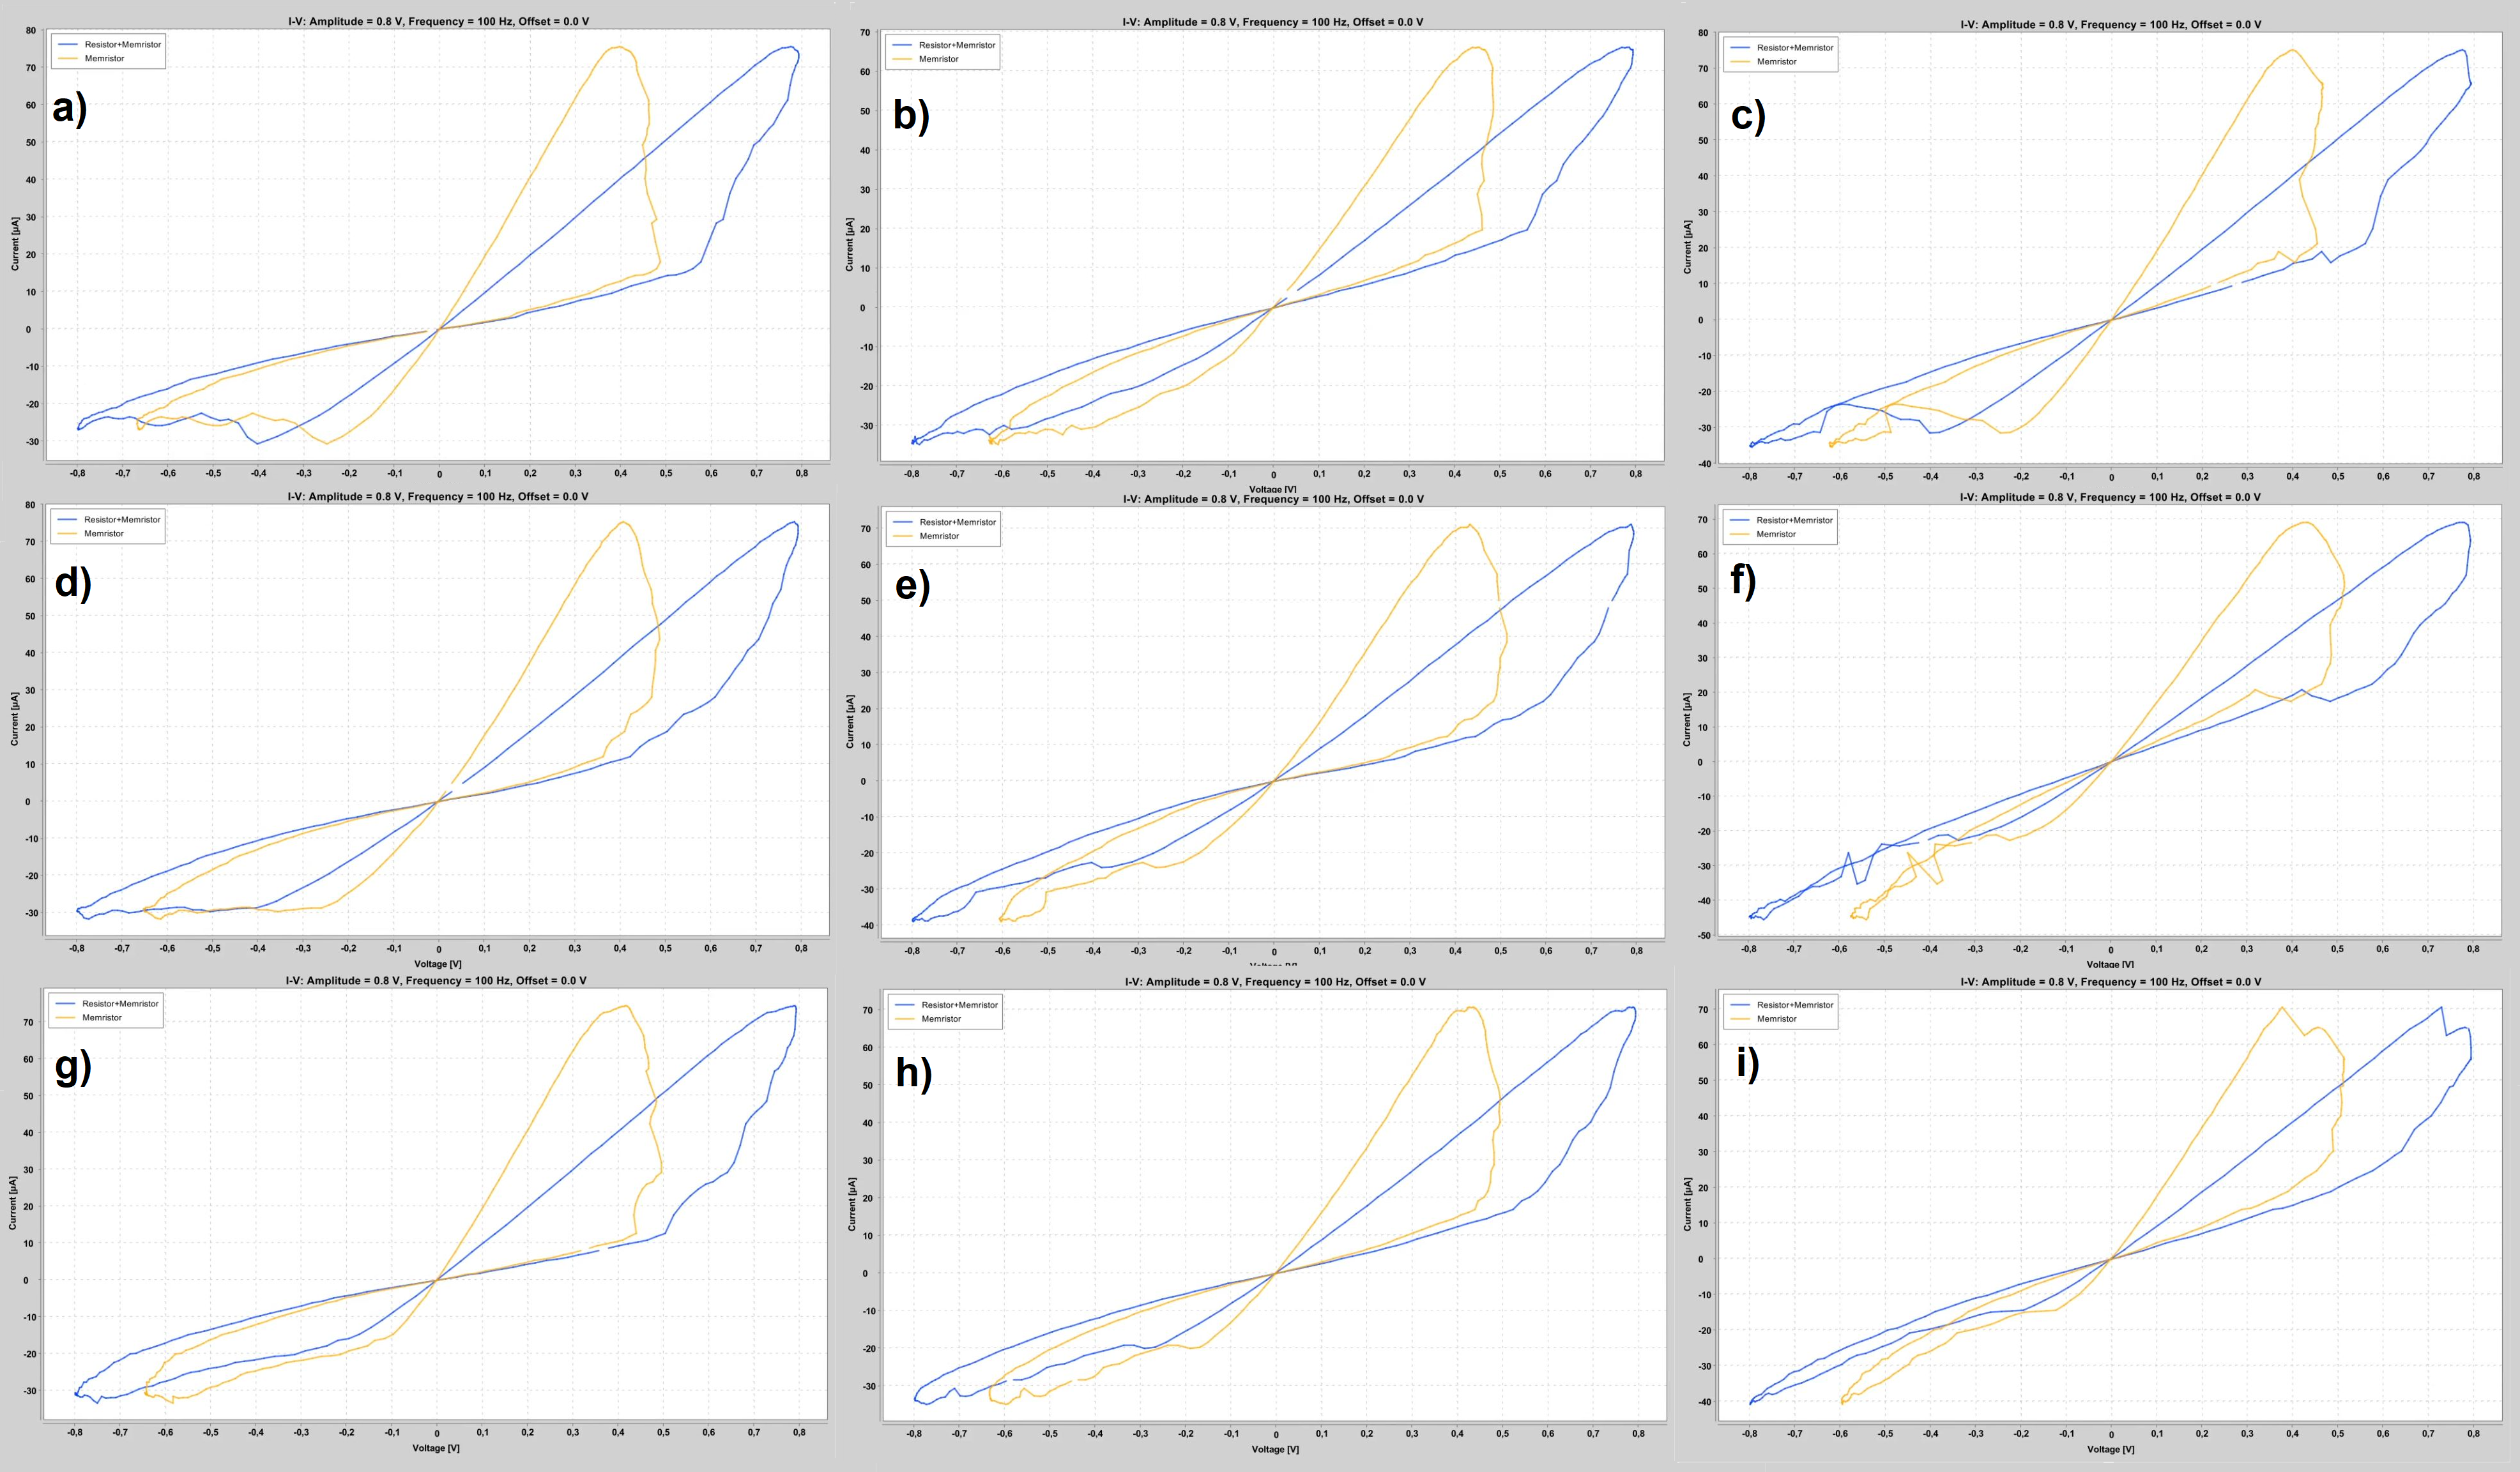
\includegraphics[width=\textwidth]{images/Hysteresen_Aufnahme.png}
  \caption{Aufnahme der Hysterese eines Memristors im Abstand von wenigen Millisekunden.}
  \label{fig:Hysteresen_Veränderung}
\end{figure}

\section{Die Benotung des Energieverbrauchs}
Dieser Abschnitt wird sich mit den Messungen zu der Energieverbrauchsnote, der \glqq t-Grade\grqq, befassen. Wie in den vorangegangenen Kapiteln schon öfter thematisiert wurde, hängt diese Note in dieser Implementierung nur von dem Threshold des Memristors ab. Aus allen Tabellen~\ref{tab:Messergebnisse_Sn},~\ref{tab:Messergebnisse_W},~\ref{tab:Messergebnisse_Cr}~und~\ref{tab:Messergebnisse_old}
ist zu erkennen, dass die t-Grade eher durchschnittlich benotet wurde, was nicht ungewöhnlich ist. Für eine t-Grade von 1 muss der Fordward Threshold im Bereich von $0.15$V und $0.205$V sein. Der Reverse Threshold muss im Bereich von $-0.05$V und $-0.08$V liegen. Diese Bereiche, speziell im Fall des Reverse Thresholds sind sehr klein, weshalb es nur ein sehr kleines Fenster für eine Note von 1 gibt. Jedoch ist bei der Messung dieser Ergebnisse aufgefallen, dass nicht nur bei den Memristoren, welche in diesem Kapitel in den Tabellen dargestellt wurden, die t-Grade meistens im Bereich zwischen 2 und 3 liegt. Es kommt insgesamt auch bei stichprobenhaften Messungen auf anderen Memristoren jeder Art, sehr selten zu einer t-Grade von 1. Es soll nun diskutiert werden, woran dies liegen kann.

\begin{figure}
  \centering
    \includegraphics[width=0.85\textwidth]{images/Threshold_Hysterese1.png}
  \caption{Hysterese eines Memristors mit unklarem Forward Threshold.}
  \label{fig:Hysteresen_Threshold}
\end{figure}

Da der Threshold in der Implementierung automatisch aus der Hystere ausgelesen wird, kann dies ein Faktor für die eher niedrigen Noten sein. Der Forward Threshold wird in der Implementierung ausgelesen, indem der erste Punkt in Teil $f_1$ gesucht wird, bei dem das Wachstum der Stromstärke zum nächsten Punkt um 50\% steigt. In Abbildung~\ref{fig:Hysteresen_Threshold} ist zu erkennen, dass die Hysterese bei ungefähr $0.22$V ein erhöhtes Wachstum der Stromstärke verzeichnet. Doch steigt die Hysterese an dieser Stelle noch nicht sofort stark an, sodass nicht mit Sicherheit gesagt werden kann, dass das Wachstum auch die 50\% Marke erreicht. Erst bei $0.32$V kann klar davon ausgegangen werden, dass die Steigung so hoch ist, dass in der Implementierung hier der Threshold gefunden wurde. Das würde die Note für den Forward Threshold in diesem Beispiel fälschlicherweise von 2 auf 4 verschlechtern.

Ein anderer möglicher Grund für eher durchschnittliche Noten für den Energieverbrauch ist die Tatsache, dass die Note aus zwei Teilnoten und ihrem Durchschnitt entsteht. Es wird einerseits der Forward Threshold und andererseits der Reverse Threshold betrachtet und jeweils mit einer Note versehen. Die Gesamtnote aus diesen beiden Teilnoten bildet dann die t-Grade. Wie in Abbildung~\ref{fig:Hysteresen_Threshold} zu erkennen ist, kann eine schlechtere Note für den Reverse Threshold eine bessere Note für den Forward Threshold ausgleichen. In der Abbildung ist der Forward Threshold bei ungefähr $0.22V$ abzulesen, für den Reverse Threshold liegt dieser bei $-0.25$V. Die Noten wären damit für den Forward Threshold bei 2 und für den Reverse Threshold bei 4. Die Gesamtnote für den Threshold würde also bei 3 liegen.

\begin{figure}
  \centering
    \includegraphics[width=0.85\textwidth]{images/Threshold_Hysterese2.png}
  \caption{Hysterese eines Memristors mit niedrigem Forward Threshold (gut) und niedrigem Reverse Threshold (schlecht).}
  \label{fig:Hysteresen_Threshold2}
\end{figure}

\section{Die Benotung der Speichergrößen}
Dieser Abschnitt wird sich mit den Messungen für die Note zur Speichergröße von Memristoren, der \glqq s-Grade\grqq\,beschäftigen. Auffällig sind hier die über alle Messungen gleichermaßen schlechten und vor allem inkonsistenten Noten für die Speichergrößen, wie in den Tabellen~\ref{tab:Messergebnisse_Sn},~\ref{tab:Messergebnisse_W},~\ref{tab:Messergebnisse_Cr}~und~\ref{tab:Messergebnisse_old}
zu erkennen ist. Wie bereits im Kapitel~\ref{sec:Chapter4} beschrieben wurde, musste für die Implementierung ein anderer Ansatz gewählt werden, als der im Konzept in Kapitel~\ref{sec:Chapter3} vorgestellte Ansatz über Pulse. Da Pulse aus unersichtlichen Gründen mit der Memristor Discovery Software nicht funktionieren, sind auch die Ergebnisse, welche mit dem Ansatz der Berechnung der Leitfähigkeit arbeiten, sehr ungenau und inkonsistent. In der aktuellen Implementierung ist es nicht möglich den Memristor in sein HRS zu bringen, somit ist in den meisten Messungen vermutlich nicht der komplette Wertebereich abgedeckt.

Auch ist der sogenannten \glqq Pulsetrain\grqq, welcher durch die von Knowm gestellte Implementierung übernommen wurde, nicht davor geschützt, dass Memristoren \glqq durchbrennen\grqq, wie es der pulsbasierte Ansatz macht. Wenn nach jedem händischen Puls eine Anzeige des aktuellen Zustands gegeben wird, ist dies auch nicht notwendig. In einem vollständig automatisierten Vorgang, wie bei der Notengeneration dieser Arbeit, kann dies jedoch zu Problemen führen, weshalb aus Vorsicht ein Counter eingebaut wurde, welcher bis zu 10 Pulse erlaubt, bei welchem sich die berechneten Leitfähigkeiten nicht merklich ändern. Danach wird der Vorgang automatisch abgebrochen. Hierbei können auch weitere Zustände \glqq übersehen\grqq\,werden.

\begin{table}
  \centering
    \begin{tabular}{l|c|c|c|c|c|c|c}
      \textbf{Mem.} & \textbf{f-Grade} & \textbf{t-Grade} & \textbf{s-Grade} & \textbf{Grade} & \textbf{minLT} & \textbf{typLT} & \textbf{maxLT} \\\hline
      Cr1          &  3               & 3                &  2               &  2.6           & Inf            & Inf            & Inf     \\
      Cr1          &  1               & 2                &  3               &  3.0           & 503173         & 1807546        & 90361405\\
      Cr1          &  3               & 4                &  2               &  3.0           & Inf            & Inf            & Inf     \\
      Cr1          &  1               & 3                &  4               &  3.6           & -8             & -421           & -842    \\
      Cr1          &  3               & 3                &  3               &  4.0           & 17             & 864            & 1729    \\
      Cr1          &  3               & 3                &  3               &  4.0           & 28450          & 1422871        & 2857942 \\
      Cr1          &  3               & 5                &  3               &  4.6           & 264            & 13248          & 26497   \\
      Cr1          &  4               & 5                &  3               &  5.0           & -17            & -852           & -1704   \\
      Cr1          &  3               & 4                &  3               &  4.6           & 95             & 4768           & 9536    \\
      Cr1          &  3               & 2                &  3               &  2.6           & 28840          & 1442041        & 2884083 \\
      Cr1          &  1               & 3                &  3               &  2.3           & Inf            & Inf            & Inf     \\
      Cr1          &  2               & 3                &  3               &  2.6           & Inf            & Inf            & Inf     \\
      Cr1          &  1               & 3                &  3               &  2.3           & Inf            & Inf            & Inf     \\
      Cr1          &  2               & 2                &  2               &  2.0           & Inf            & Inf            & Inf     \\
    \end{tabular}
  \caption{Ausschnitt der Messergebnisse von wiederholten Messungen auf einem Chrom (Cr) Memristor der neuen Generation.}
  \label{tab:Messergebnisse_Cr}
\end{table}

Ein weiterer Grund für schlechte Noten ist die allgemein sehr strenge Benotung der Speichergrößen. Selbst bei einem vollständig funktionsfähigen und getesteten Ansatz zur Speichergrößenbestimmung wäre nicht sicher, ob einer der Knowm Memristoren 16 oder mehr Zustände erreichen kann. Die meisten aktuellen Memristoren von Knowm können aus Erfahrung in händischen Test zwischen 2.5 und 3.5 Bit codieren. Mehr als 16 Zustände wären bereits in der vier Bit Reichweite, was ein im Vergleich zum Durchschnitt wirklich guten Memristor darstellen würde.

Des Weiteren ist hier bereits etwas anzumerken, was im folgenden Abschnitt~\ref{sec:Restlebensdauer} noch näher beschrieben werden soll. Der Unterschied zwischen dem gemessenen HRS und LRS ist für nahezu alle Messreihen sehr nahe aneinander, manchmal sogar negativ. Das wirft jedoch die Frage auf, wie der leitfähigkeitsbasierte Ansatz, ohne die Zustände merklich zu ändern, verschiedene Leitfähigkeiten berechnet. Dafür müssten weitere Tests und Messreihen mit dem Ansatz gemacht werden, welche es aus Zeitgründen nicht mehr in diese Arbeit geschafft haben.

\section{Die Restlebensdauer}
\label{sec:Restlebensdauer}
Dieser Abschnitt wird sich mit der Bestimmung der Restlebensdauer von Memristoren beschäftigen. Auch hier ist wie im vorherigen Abschnitt auffällig, dass die approximierte Restlebensdauer der Memristoren sehr stark zwischen den einzelnen Messungen schwankt. Dies lässt sich jedoch nicht direkt auf die Berechnung der approximierten Restlebensdauer zurückführen. Diese wurde in dem Kapitel~\ref{sec:Chapter4} beschrieben und näher erklärt. Damit diese Art von Approximation funktionieren kann, muss jedoch zuerst die Messung des HRS und LRS funktionieren.

Wie in den letzten Abschnitten und Kapiteln mehrfach erwähnt wurde, ist dies aufgrund der nicht funktionierenden Pulse jedoch nicht möglich. In nahezu allen Messungen liegen HRS und LRS dadurch sehr nahe aneinender. In den Fällen, in welchen eine negative Restlebensdauer ausgerechnet und zurückgegeben wird, liegt der LRS anhand der Messung sogar knapp über dem HRS. Dazu kommt noch, dass dadurch, dass die beiden Zustände fast immer sehr nahe aneinander liegen, immer der 10\% Restlebensdauer Bereich erreicht wird, was die Gesamtnote immer um eine Note verschlechtert. Dies ist naürlich nicht der Fall, wenn die Restlebensdauer \glqq Inf\grqq\,ist.


\begin{table}
  \centering
    \begin{tabular}{l|c|c|c|c|c|c|c}
      \textbf{Mem.} & \textbf{f-Grade} & \textbf{t-Grade} & \textbf{s-Grade} & \textbf{Grade} & \textbf{minLT} & \textbf{typLT} & \textbf{maxLT} \\\hline
      oldW1          &  3               & 3                &  5               &  4.6           & -38000         & -77400         & -3871676\\
      oldW1          &  2               & 3                &  5               &  3.3           & Inf            & Inf            & Inf     \\
      oldW1          &  2               & 3                &  5               &  3.3           & Inf            & Inf            & Inf     \\
      oldW1          &  4               & 4                &  5               &  5.3           & 996657         & 19993315       & 999665757\\
      oldW1          &  3               & 2                &  5               &  3.3           & Inf            & Inf            & Inf     \\
      oldW1          &  1               & 3                &  5               &  3.0           & Inf            & Inf            & Inf     \\
      oldW1          &  3               & 3                &  5               &  4.6           & 0              & 0              & 0    \\
      oldW1          &  2               & 3                &  5               &  3.3           & Inf            & Inf            & Inf     \\
      oldW1          &  1               & 3                &  6               &  4.3           & 14860          & 29720          & 1486036 \\
      oldW2          &  4               & 3                &  6               &  4.3           & Inf            & Inf            & Inf     \\
      oldW2          &  4               & 3                &  6               &  4.3           & Inf            & Inf            & Inf     \\
      oldW2          &  4               & 3                &  6               &  4.3           & Inf            & Inf            & Inf     \\
      oldW2          &  4               & 3                &  6               &  4.3           & Inf            & Inf            & Inf     \\
      oldW2          &  4               & 3                &  6               &  5.3           & -5944          & -11889         & -594456 \\
    \end{tabular}
  \caption{Ausschnitt der Messergebnisse von wiederholten Messungen auf Wolfram (W) Memristoren der alten Generation.}
  \label{tab:Messergebnisse_old}
\end{table}

Es fällt bei den Messungen auf, dass einige Angaben der Restlebensdauer mit der Bezeichnung \glqq Inf\grqq\,angegeben sind. Dies geschieht nicht in der Konsole und Ausgabe des Programms. \glqq Inf\grqq\,ist in den Tabellen dieses Kapitels vielmehr eine Abkürzung der Zahl $9223372036854775807$, welche für die minimalen, typischen und maximalen Restlebensdauer in der Konsole ausgegeben wird. Da $5000000000$ als maximale Restlebensdauer definiert ist, kann eine solche Restlebensdauer nach Berechnungsvorschrift gar nicht zustande kommen. Wieso sie dann trotzdem angezeigt wird, klärt der folgende Absatz.

Die durch die Memristor Discovery Software gegebene Funktion mit dem Namen \lstinline[columns=fixed]{getSwitchResistancekOhm}
gibt den aktuellen Widerstand des mittels eines \glqq Switch-Buttons\grqq\,ausgewählten Memristors wieder. Der zurückgegebene Widerstand wird jedoch in einigen nicht ersichtlichen Fällen, am häufigsten jedoch, wenn der Memristor in einen hochohmigeren Bereich liegt, nicht als spezifischer Wert, sondern als \glqq Infinity\grqq\,zurückgegeben. Ist dies der Fall, wenn HRS oder LRS gemessen werden, so wird die Berechnung der Restlebensdauer mit \glqq Unendlich\grqq\,als Eingabe berechnet. Bei der Berechnung kommt also in Folge daraus wieder Unendlich heraus, welches mit $9223372036854775807$ ausgegeben wird, da die Restlebensdauer als Datentyp Long gespeichert wird und es sich dabei um den maximalen Wert eines Longs handelt.

\begin{table}
  \centering
    \begin{tabular}{l|c|c||l|c|c}
      \textbf{Mem.} & \textbf{Note} & \textbf{Zeit (in s)} & \textbf{Mem.} & \textbf{Note} & \textbf{Zeit (in s)} \\
      Sn            & 2.3           & 7,46                 & Cr            & 3.3           & 6,12     \\
      Sn            & 4.3           & 9,83                 & Cr            & 3.3           & 8,38     \\
      Sn            & 3.6           & 9,02                 & Cr            & 3.6           & 8,43     \\
      Sn            & 4.6           & 6,35                 & Cr            & 3.3           & 6,50     \\
      Sn            & 4.3           & 7,72                 & Cr            & 1.6           & 7,40     \\
      Sn            & 3.0           & 5,59                 & Cr            & 2.6           & 5,86     \\
      Sn            & 4.0           & 10,26                & Cr            & 3.3           & 8,69     \\
      Sn            & 2.6           & 5,89                 & Cr            & 3.6           & 7,13     \\
      Sn            & 5.0           & 5,86                 & Cr            & 1.6           & 9,10     \\
      Sn            & 4.0           & 9,07                 & Cr            & 3.3           & 6,40     \\
      Sn            & 3.6           & 7,96                 & Cr            & 1.6           & 6,55     \\
      Sn            & 4.0           & 9,50                 & Cr            & 2.0           & 6,82     \\
      Sn            & 4.6           & 6,29                 & Cr            & 2.6           & 8,29     \\
      Sn            & 3.6           & 9,39                 & Cr            & 3.6           & 6,65     \\
      Sn            & 4.3           & 5,28                 & Cr            & 1.6           & 7,13     \\
      Sn            & 3.3           & 7,53                 & Cr            & 3.6           & 5,66     \\
      Sn            & 3.0           & 10,93                & Cr            & 3.3           & 7,67     \\
      Sn            & 4.3           & 10,65                & Cr            & 3.3           & 6,59     \\
      Sn            & 4.6           & 9,65                 & Cr            & 3.3           & 6,78     \\
      Sn            & 4.6           & 7,45                 & Cr            & 2.6           & 6,97     \\
      Sn            & 4.3           & 9,45                 & Cr            & 2.6           & 6,33     \\
      Sn            & 4.6           & 7,56                 & Cr            & 2.0           & 7,91     \\
      Av.           & 3.9           & 8,12                 & Av.           & 2.8           & 7,15     \\
    \end{tabular}
  \caption{Laufzeit eines Durchlaufs zur Qualitätsbestimmung von Memristoren vom Material Zinn und Chrom der neuen Generation.}
  \label{tab:Laufzeit}
\end{table}

Für den Fall, dass sowohl das pulsbasierte Finden von HRS und LRS funktioniert und es einen Weg gibt, den Widerstand des Memristors als konkreten Wert zurückzugeben anstatt in einigen Fällen \glqq Inf\grqq\,als Messung zu erhalten, müsste für die Lebensdauer von Memristoren noch einige Messungen und Test durchgeführt werden. Dabei müsste überprüft werden, ob sich die approximierte Restlebensdauer des Memristors durch wiederholtes Schreiben über einen längeren Zeitraum verringert. Im aktuellen Zustand der Implementierung ist dies noch nicht möglich.

Auch lässt sich über den Zusammenhang zwischen Lebensdauer und Qualität keine Aussage treffen, da die Messergebnisse aus genannten Gründen nicht aussagekräftig genug sind.

\section{Die Laufzeit der Implementierung}

Dieser Abschnitt wird sich mit dem Laufzeit der Implementierung auseinandersetzen. Aus der Messreihe in Tabellen~\ref{tab:Laufzeit}~und~\ref{tab:Laufzeit2} ist zu erkennen, dass sich die Zeit zwischen den Durchläufen teilweise sehr stark unterscheidet. Auffallend ist die erste Messung mit dem Wolframmemristor der neuen Generation. Die $20.39$s, welche dabei benötigt wurden, sind mit großem Abstand die am längsten benötigte Zeit. Dabei handelt es sich um die erste Messung der gesamten Messreihe über alle Memristorarten. Es konnte jedoch noch nicht rekonstruiert werden, ob die erste Messung auf den Memristoren immer länger dauert, als die nachfolgenden Messungen.

Auffällig ist außerdem, dass die durchschnittliche Dauer der Qualitätsbestimmung für die Chrom Memristoren eindeutig am niedrigsten von allen Memristortypen ist. Daraus lässt sich folgern, dass Chrom Memristoren dafür, dass sie einen höheren Threshold und eine kürzere Gesamtlebensdauer haben (siehe~\cite{knowm_comp_2019}), eine schnellere Lese- und Schreibgeschwindigkeit besitzen.

\begin{table}
  \centering
    \begin{tabular}{l|c|c||l|c|c}
      \textbf{Mem.} & \textbf{Note} & \textbf{Zeit (in s)} & \textbf{Mem.} & \textbf{Note} & \textbf{Zeit (in s)} \\
      W$_{\text{new}}$            & 4.0           & 20,39                & W$_{\text{old}}$            & 4.3           & 5,75     \\
      W$_{\text{new}}$            & 3.3           & 12,79                & W$_{\text{old}}$            & 5.3           & 9,48     \\
      W$_{\text{new}}$            & 4.0           & 14,53                & W$_{\text{old}}$            & 5.0           & 5,08\footnote{\label{tab_footnote}Vorzeitiger Abbruch (Programm wurde nicht vollständig durchgeführt)}     \\
      W$_{\text{new}}$            & 3.3           & 10,96                & W$_{\text{old}}$            & 5.3           & 8,58     \\
      W$_{\text{new}}$            & 3.6           & 12,36                & W$_{\text{old}}$            & 3.0           & 8,42     \\
      W$_{\text{new}}$            & 3.3           & 8,88                 & W$_{\text{old}}$            & 4.3           & 7,43     \\
      W$_{\text{new}}$            & 2.0           & 7,88                 & W$_{\text{old}}$            & 3.0           & 7,90     \\
      W$_{\text{new}}$            & 3.0           & 4,65                 & W$_{\text{old}}$            & 4.3           & 11,30    \\
      W$_{\text{new}}$            & 1.6           & 8,02                 & W$_{\text{old}}$            & 4.3           & 10,78    \\
      W$_{\text{new}}$            & 3.3           & 7,55                 & W$_{\text{old}}$            & 5.3           & 8,63     \\
      W$_{\text{new}}$            & 2.3           & 7,23                 & W$_{\text{old}}$            & 5.3           & 6,52     \\
      W$_{\text{new}}$            & 3.0           & 8,53                 & W$_{\text{old}}$            & 4.3           & 10,09    \\
      W$_{\text{new}}$            & 3.3           & 10,05                & W$_{\text{old}}$            & 3.6           & 14,26    \\
      W$_{\text{new}}$            & 3.3           & 5,42                 & W$_{\text{old}}$            & 3.3           & 7,03     \\
      W$_{\text{new}}$            & 4.0           & 6,09                 & W$_{\text{old}}$            & 5.3           & 6,83     \\
      W$_{\text{new}}$            & 1.6           & 6,18                 & W$_{\text{old}}$            & 3.6           & 9,43     \\
      W$_{\text{new}}$            & 3.0           & 8,20                 & W$_{\text{old}}$            & 3.6           & 10,03    \\
      W$_{\text{new}}$            & 3.6           & 7,62                 & W$_{\text{old}}$            & 4.0           & 8,43     \\
      W$_{\text{new}}$            & 3.6           & 9,83                 & W$_{\text{old}}$            & 5.3           & 8,23     \\
      W$_{\text{new}}$            & 3.6           & 9,26                 & W$_{\text{old}}$            & 5.0           & 7,68\footref{tab_footnote}     \\
      W$_{\text{new}}$            & 2.0           & 7,20                 & W$_{\text{old}}$            & 5.0           & 2.16\footref{tab_footnote}     \\
      W$_{\text{new}}$            & 3.6           & 8,18                 & W$_{\text{old}}$            & 4.0           & 8,55     \\
      Av.                         & 3.1           & 9,17                 & Av.                         & 4.3           & 8,20     \\
    \end{tabular}
  \caption{Laufzeit eines Durchlaufs zur Qualitätsbestimmung von Memristoren vom Material Wolfram der neuen und alten Generation.}
  \label{tab:Laufzeit2}
\end{table}

Für alle Memristortypen lässt sich aus den Tabellen~\ref{tab:Laufzeit}~und~\ref{tab:Laufzeit2} außerdem entnehmen, dass die Note keinerlei Einfluss auf die Laufzeit des Programms hat. Trotzdem ist die Zeit, wie bereits beschrieben, sehr unterschiedlich in den verschiedenen Messungen. Dies lässt sich darauf zurückführen, dass es im Programm öfter zu Wiederholungen von Messungen kommt, wenn diese unvollständig oder verschoben aufgenommen werden. Nur wenn eine Messung mehrmals hintereinander fehlschlägt, wird abgebrochen. Die Folge daraus ist, dass bei einigen Messungen eine erhöhte Anzahl an Messwiederholungen stattfinden. Wenn ein funktionierender Memristor vorliegt, wird im Fall, dass die Messung fehlschlägt, in einer der darauf folgenden Messwiederholungen eine valide Messung vorgenommen und der Vorgang zur Qualitätsbestimmung kann weiter durchgeführt werden. In Folge dessen steigt die Bearbeitungszeit jedoch an. Somit entstehen sehr unterschiedliche Bearbeitungszeiten für die verschiedenen Messungen auf den Memristortypen.

\section{Der Einfluss des Materials auf die Qualität}
In diesem Abschnitt soll es abschließend um den Einfluss des Materials auf die Qualität gehen. Aufgrund der in diesem Kapitel beschriebene Probleme, können keine klaren Aussagen über den Einfluss des Materials auf die Qualität getroffen werden. Doch ist auffällig, dass der Zinnmemristor in Tabelle~\ref{tab:Laufzeit} von der durchschnittlichen Qualität der Messreihe eher dem Memristor der alten Generation ähnelt, während die Memristoren aus dem Material Chrom aus Tabelle~\ref{tab:Laufzeit} und dem Material Wolfram der neuen Generation aus Tabelle~\ref{tab:Laufzeit2} mit ihrer durchschnittlichen Qualität näher aneinander liegen. Auch fällt auf, dass die durchschnittliche Laufzeit zum Kategorisieren der Memristoren für die Wolfram Memristoren beider Generationen und für den Zinn Memristor ähnlich lange ist. Der Wolfram Memristor der neuen Generation sticht durch die ungewöhnlich lange Messung zu Beginn zwar im Durchschnitt mit fast einer Sekunde heraus, wenn der Durchschnitt jedoch aus den anderen 21 Messwerten errechnet wird und die 20,39s zu Beginn ignoriert werden, errechnet sich eine durchschnittliche Laufzeit von 8,6s. Der Chrom Memristor dagegen scheint mit keiner einzigen Laufzeit von über 10 Sekunden und einem Durchschnitt von 7,15s schneller als die Memristoren anderer Materialen zu sein.

%% ----------------------------------
%%   Kap06---Zusammenfassung.tex
%% ----------------------------------

%% Zusammenfassung der wesentlichen Punkte und
%% Ausblick, was man mit dem nun existierenden Prototypen alles anstellen könnte (aber zu viel für diese Arbeit gewesen wäre)

\chapter{Zusammenfassung}
\label{sec:Chapter6}
Dieses Kapitel stellt eine Zusammenfassung der gesamten Arbeit dar. Dabei wird speziell auf die Zielsetzung in Kapitel~\ref{sec:Chapter1} eingegangen. In dieser Arbeit wurde ein allgemeiner Überblick über Memristoren und über wissenschaftliche Paper mit Ähnlichkeiten zu dieser Arbeit gegeben. Dabei wurde festgestellt, dass es keine wissenschaftlichen Arbeiten gibt, die ein allgemeines Qualitätsmaß für die Betrachtung von einzelnen Memristoren aufstellen. Auch wurde festgestellt, dass ein solches Qualitätsmaß für viele verschiedene Anwendungsgebiete von Nutzen ist.

Das Kapitel~\ref{sec:Chapter3} liefert eine theoretische Betrachtung eines Qualitätsmaßes auf Grundlage von Formbarkeit, Energieverbrauch, Speichergröße und Lebensdauer von Memristoren. Dabei werden Ansätze und Konzepte vorgestellt, welche verwendet werden können, um die genannten Faktoren in ein Qualitätsmaß einzubinden. Auch der Einfluss des Materials wird thematisiert und der Vergleich zwischen zwei Memristoren wird beschrieben, obwohl dieser in der Implementierung nicht umgesetzt, sondern rein theoretisch in diesem Abschnitt im dritten Kapitel diskutiert wird.

Da Memristoren in ihrem aktuellen Zustand noch zu fehlerbehaftet sind, um problemlos zu arbeiten, kam es in der Realisierung des Konzepts zu einigen Schwierigkeiten. Die Forschungsumgebung \glqq Memristor Discovery\grqq\,von Knowm Inc. hat bei Spannungspulsen auf Memristoren auch noch schwerwiegende Probleme.

Die Bestimmung der Formbarkeit hat grundlegend gut funktioniert. Probleme, welche dabei auftraten, sind Messungenauigkeiten, welche sich beim aktuellen Entwicklungsstand des Memristor Discovery Board 2, nicht verhindern lassen. Durch die Pulse, welche in der Memristor Discovery Software nicht funktionieren, kam es bei den anderen Funktionalitäten der Implementierung zu größeren Problemen.

Die Energieverbrauchsnote musste durch die alleinige Betrachtung des Thresholds vereinfacht werden, da der niedrigst mögliche Widerstandsbereich nicht klar eruiert werden konnte. Da der Threshold jedoch eine sehr große Rolle im Energieverbrauch spielt, wird das Qualitätskriterium des Energieverbrauchs in der Implementierung trotzdem abgedeckt.

Die Speichergrößenbestimmung wurde aufgrund von in der Arbeit beschriebenen Problemen durch eine Notlösung implementiert. Ohne weitere Tests und Verbesserungen wird  nicht empfohlen, diese in der Praxis zur Klassifikation der Speichergröße zu verwenden, da nicht komplett sicher gestellt ist, dass der Memristor nicht durch Pulse im niedrigohmigen Bereich beschädigt wird. Der theoretische Ablauf zur Speichergrößenbestimmung von Memristoren wird trotzdem geliefert und erklärt.

Auch die Implementierung der Approximation der Restlebensdauer von Memristoren leidet stark darunter, dass es in der Implementierung nicht möglich ist, den LRS und den HRS zu bestimmen. Die Berechnung, welche auf Basis der wissenschaftlichen Arbeit~\cite{stat_lifetime} vorgenommen wird, kann ohne Bestimmung von HRS und LRS keine richtigen Ergebnisse liefern. Die Formeln für die Approximation lassen sich jedoch sehr leicht in ein System übernehmen, in dem HRS und LRS ausgemessen werden können.

Diese Arbeit bietet trotz der Probleme einen auf theoretischer Ebene ausgereiften Ansatz zur automatischen Qualitätsbestimmung von Memristoren. Mit genügend Zeit und Aufwand kann die Implementierung ohne Knowms Memristor Discovery Software implementiert werden, wodurch sie funktionsfähig sein sollte.


\bibliographystyle{geralpha}
%\bibliographystyle{gerabbrv}
%gerabbrv macht das so wie jetzt, nur mit Zahlen statt der Buchstabenkombination
%\bibliographystyle{unsrtdin}
\bibliography{./otherincludes/Referenzen}

\thispagestyle{empty}
\null \newpage

\appendix
%%% ----------------------------------
%%   AnhA---Material und Methoden.tex
%% ----------------------------------

%% Anhänge: Z.B. längere Listingauszüge, Schaltbilder, etc.

\chapter{Anhang\"uberschrift}
\label{sec:ChapterA}


%------------------------------------------------------------------------
%\textcolor{red}{\textbf{roter Text}}
%% ------------------------------------------------------------------------

\end{document}
